\documentclass[11pt, a4paper, oneside]{book}
\usepackage[margin=2.5cm]{geometry}

\usepackage[portuguese]{babel}

\usepackage[utf8]{inputenc}
\usepackage[x11names,table]{xcolor}
\usepackage{graphicx}
\usepackage[toc,page]{appendix}

\usepackage[binary-units=true]{siunitx}
\sisetup{
    range-phrase=--,
    range-units=single,
    group-separator = {\,}
}
\DeclareSIUnit{\euro}{\mbox{€}}
\usepackage{svg}
\usepackage[hyphens]{url}
\usepackage{hyperref}
\usepackage{caption}
\usepackage{subcaption}
\usepackage{glossaries}
\usepackage{titlepic}
\usepackage{lmodern}
\renewcommand{\familydefault}{\sfdefault}
\usepackage{pdfpages}
\usepackage{fancyhdr}
\usepackage{tikz}
\usepackage{titlesec}
\usepackage{enumitem}
\usepackage{mdframed}
\usepackage{lipsum}

\usepackage{pifont}
\newcommand*\checkmark{%
  \ding{52}%
}

\setlength{\parskip}{0.20\baselineskip}%

\newcommand{\email}[1]{\texttt{#1}}

\pagestyle{fancy}
\fancyhf{}
\renewcommand{\headrulewidth}{0pt}
\fancyhead[R]{
\includegraphics[width=2.0em]{img/recycle-it.png}}
\fancyfoot[C]{\thepage}
\setlength{\headheight}{28pt}
\setlength{\headsep}{10pt}

\definecolor{ourdarkgreen}{HTML}{216942}
\definecolor{ourgreen}{RGB}{44, 142, 90}
\definecolor{ourlightgreen}{HTML}{4AB27B}
\definecolor{ourlightestgreen}{HTML}{7FBF9D}
\definecolor{strengthgreen}{HTML}{00e804}

\titleformat
{name=\chapter,numberless} % command
[block] % shape
{
    \begin{tikzpicture}[remember picture,overlay]
        \fill[ourgreen](-25mm,22mm) rectangle ++(218mm, -30mm);
    \end{tikzpicture}
    \bfseries\Large
} % format
{
} % label
{0.5ex} % sep
{
    \fontsize{30}{30}\selectfont
    \hspace{-10.3mm}
    \color{white}
} % before-code
[
] % after-code
\titlespacing*{name=\chapter,numberless}{0pt}{-1mm}{20mm}

\titleformat
{\chapter} % command
[block] % shape
{
    \begin{tikzpicture}[remember picture,overlay]
        \fill[ourgreen](-25mm,35.5mm) rectangle ++(218mm, -50mm);
        \fill[white](-25mm,27.5mm) rectangle ++(34mm, -34mm);
        \draw(-3mm,8.5mm) node[color=ourgreen, align=left] {\bfseries \fontsize{70}{70}\selectfont \thechapter};
    \end{tikzpicture}
    \bfseries\Large
} % format
{
} % label
{0.5ex} % sep
{
    \fontsize{30}{30}\selectfont
    \hspace{8mm}
    \color{white}
} % before-code
[
] % after-code
\titlespacing*{\chapter}{0pt}{14mm}{25mm}

\makeatletter
\def\printauthor{{\@author}}
\makeatother

\makeatletter
\def\printtitle{{\@title}}
\makeatother

\makeatletter
\def\printdate{{\@date}}
\makeatother

\makeatletter
\def\printinstitution{%
Mestrado Integrado em Engenharia Informática e Computação \\
3º ano, 2º semestre \\
Proficiência Pessoal e Interpessoal
}
\makeatother

% Copyright page
\newenvironment{secondpage}{
    \clearpage\null\vfill
    \thispagestyle{empty}
    \begin{minipage}[b]{0.9\textwidth}
        \footnotesize\raggedright
        \setlength{\parskip}{0.5\baselineskip}
}{
    \end{minipage}
    \vspace*{2\baselineskip}
}

% Metadata
\title{
\includegraphics[scale=0.2]{img/recycle-it-full-white.png}}
\author{
    \hspace{-3.4mm}
    \begin{tabular}{@{} l l @{}}
        Diogo Miguel Ferreira Rodrigues & (\email{up201806429@edu.fe.up.pt}) \\
        Iohan Xavier Sardinha Dutra Soares & (\email{up201801011@edu.fe.up.pt}) \\
        João António Cardoso Vieira e Basto de Sousa & (\email{up201806613@edu.fe.up.pt}) \\
        Pedro Daniel Fernandes Ferreira & (\email{up201806506@edu.fe.up.pt}) \\
        Pedro Varandas da Costa Azevedo da Ponte & (\email{up201809694@edu.fe.up.pt})
    \end{tabular}
}
\date{6 de Junho de 2021}

\makeglossaries
\newglossaryentry{rsu}{
    name=resíduo sólido urbano,
    description={Designado abreviadamente de RSU, é um objeto ou substância sólida que, na sua condição atual, não possui utilidade para quem o detém, pelo que deve ser descartado de forma adequada. Não possuir utilidade para quem o detém não significa que não tenha valor económico: não só as matérias-primas do qual o RSU é feito possuem geralmente valor económico, como o RSU pode ser útil a outra pessoa ou empresa que seja capaz de reutilizar/reciclar o RSU. Neste documento os termos "lixo" e "resíduos" são usados como sinónimos de RSU}
}
\newglossaryentry{lixo}{
    name=lixo,
    description={Equivalente a resíduo sólido urbano}
}
\newglossaryentry{entidade gestora}{
    name=entidade gestora,
    description={Entidade que gere a recolha e tratamento dos resíduos sólidos urbanos numa determinada zona; pode-se tratar, por exemplo, de um município, de uma empresa municipal especializada, ou de uma entidade trans-municipal \cite{dl-152d-2017}}
}
\newglossaryentry{justica ambiental}{
    name=justiça ambiental,
    description={Termo utilizado para enquadrar os problemas ambientais (aquecimento global, poluição, destruição de habitat) como questões éticas e políticas, e não apenas como questões ambientais ou físicas. Geralmente refere-se à forma injusta como diferentes países e classes sociais são afetados por problemas ambientais originados pela forma como a sociedade de consumo mundial opera, pelo que a justiça ambiental é atingida quando cada pessoa é responsabilizada, tributada ou processada judicialmente em proporção com o impacto negativo que tem no meio ambiente}
}

\usepackage[utf8]{inputenc}
\usepackage{array, booktabs}
\usepackage{graphicx}

\newcommand{\foo}{\color{ourgreen}\makebox[0pt]{\Large$\bullet$}\hskip-1pt\vrule width 2pt\hspace{\labelsep}}

\linespread{1.075}
\begin{document}

\begin{titlepage}
    \begin{tikzpicture}[remember picture,overlay]
        \begin{scope}[shift={(-31mm, 10mm)}]
            \draw[fill=ourgreen, ourgreen]
                  (0, 0) rectangle ++(210mm, -52mm);
        \end{scope}
    \end{tikzpicture}
    \begin{tikzpicture}[remember picture,overlay]
        \begin{scope}[shift={(177.7mm, 10mm)}, scale=2]
            \draw[fill=ourdarkgreen, ourdarkgreen]
                  (0, 0) rectangle ++(-1, -1);
            \draw[fill=ourlightestgreen, ourlightestgreen]
                  (-1, +0) node[]{} --
                ++(-1, +0) node[]{} --
                ++(+0, -1) node[]{} -- cycle;
            \draw[fill=ourlightgreen, ourlightgreen]
                  (-1, +0) node[]{} --
                ++(+0, -1) node[]{} --
                ++(-1, +0) node[]{} -- cycle;
            \draw[fill=ourdarkgreen, ourdarkgreen]
                  (-2, +0) node[]{} --
                ++(+0, -1) node[]{} --
                ++(-1, +1) node[]{} -- cycle;
            \draw[fill=ourlightestgreen, ourlightestgreen]
                  (-1, -1) node[]{} --
                ++(+1, +0) node[]{} --
                ++(+0, -1) node[]{} -- cycle;
        \end{scope}
    \end{tikzpicture}
    \begin{tikzpicture}[remember picture,overlay]
        \draw(-15mm,-15mm) node[anchor=west] {\printtitle};
    \end{tikzpicture}
    \begin{tikzpicture}[remember picture,overlay]
        \draw(-15mm,-70mm) node[anchor=west] {\bfseries \Huge Relatório do projeto};
    \end{tikzpicture}
    \begin{tikzpicture}[remember picture,overlay]
        \draw(-15mm,-97mm) node[anchor=west, align=left] {
            \printauthor
        };
    \end{tikzpicture}
    \begin{tikzpicture}[remember picture,overlay]
        \draw(-17mm,-115mm) node[anchor=north west, align=left] {
            \printinstitution
        };
    \end{tikzpicture}
    \begin{tikzpicture}[remember picture,overlay]
        \draw(+70mm,-250mm) node[anchor=south, align=center] {
            % \includesvg[scale=0.3]{img/minerva.svg} \\
            
\includegraphics[scale=0.4]{img/feup.png} \\[2em]
        
            % Faculdade de Engenharia da Universidade do Porto \\
            Porto, Portugal \\
            \printdate
        };
    \end{tikzpicture}
\end{titlepage}
\pagecolor{white}
        
\begin{secondpage}
    Copyright \copyright 2021--\the\year\ Diogo Rodrigues, João António Sousa, Pedro Ferreira, Pedro Ponte, Iohan Soares\par
    É permitida a cópia e redistribuição deste documento sob os termos da licença pública
    \href{https://creativecommons.org/licenses/by-nc-nd/4.0/}{Creative Commons Attribution-NonCommercial-NoDerivatives 4.0 International}.\par
    
    \vspace{2em}
    
    Autores: \par
    \begin{tabular}{@{} l l @{}}
        Diogo Miguel Ferreira Rodrigues & (\email{up201806429@edu.fe.up.pt}) \\
        Iohan Xavier Sardinha Dutra Soares & (\email{up201801011@edu.fe.up.pt}) \\
        João António Cardoso Vieira e Basto de Sousa & (\email{up201806613@edu.fe.up.pt}) \\
        Pedro Daniel Fernandes Ferreira & (\email{up201806506@edu.fe.up.pt}) \\
        Pedro Varandas da Costa Azevedo da Ponte & (\email{up201809694@edu.fe.up.pt})
    \end{tabular}\par
    
    \vspace{2em}

    Realizado sob supervisão da Professora Fernanda Maria dos Santos Teixeira Torres.
\end{secondpage}

\frontmatter

{
\linespread{1.000}

\tableofcontents
}

\printglossaries
\glsaddallunused

\mainmatter

\chapter{Introdução}

A RecycleIt é um sistema de informação que se enquadra na temática da separação e recolha de resíduos, sendo caracterizada por duas funcionalidades principais: sistema de informação dirigido às entidades de resíduos e uma aplicação móvel/web app a ser utilizada pelo cidadão comum.

Hoje em dia, existe uma grande preocupação com a separação de resíduos. Contudo, os incentivos para este comportamento não são intrinsecamente atrativos. De forma geral, a única recompensa garantida é o reconhecimento próprio de se estar a não contribuir para um aumento do desperdício e consequente poluição do ambiente. As taxas de resíduos sólidos não têm em conta esta situação, não havendo nenhum impacto direto no ato de separar corretamente.

O principal objetivo é o aumento da separação correta dos resíduos por parte dos cidadãos, recompensando os "participantes"{} com parte das receitas que a entidade gestora de resíduos obtém com esta mudança de comportamentos, ou seja, originaria não só benefícios para o ambiente como também para as pessoas. Além disso, este sistema permite a implementação de um sistema PAYT (\textit{pay as you throw}), também conhecido como o princípio do poluidor-pagador, promovendo a justiça ambiental a partir das atitudes das pessoas.

\chapter{Revisão bibliográfica}

\section{Legislação e Evidência}

Ao longo dos anos, cada vez mais têm sido abordadas temáticas relacionadas com o ambiente. A reciclagem, a redução dos desperdícios, a gestão de resíduos e o seu tratamento e recolha são assuntos de que se houve falar quase diariamente, existindo trabalhos constantes neste âmbito não só a nível europeu, como também a nível nacional.
Segundo um relatório do eurostat \cite{waste-generation-2018}, em 2018, na União Europeia a quantidade de resíduos gerados totalizava as 2337 milhões de toneladas, sendo sensivelmente 8\% deste proveniente de um contexto doméstico, ou seja, 186 milhões de toneladas. Nesse mesmo ano, 2169 milhões de toneladas foram alvo de tratamento, 54.6\% desses recuperados o que representa um aumento de 8.7\% face aos 45.9\% de 2004. Contudo, é de notar que não se pode comparar diretamente estes números uma vez que os dados dos resíduos tratados não incluem as quantidades que foram exportadas, mas incluem as que foram importadas.
De acordo uma vez mais com o eurostat, em média, em 2019, apenas 47.7\% dos resíduos municipais (i.e. resíduos coletados e tratados pelos municípios) foram reciclados, situando-se Portugal bastante abaixo da média com apenas 28.9\% \cite{recycling-municipal-waste}.

De relevo, ainda a nível europeu, importa também salientar a diretiva 2008/98/CE relativa a esta matéria de gestão de resíduos que estabeleceu o quadro legal para o tratamento dos resíduos na União Europeia. Esta é caracterizada, entre outros, pelos seguintes pontos:
\begin{itemize}
    \itemsep0em
    \item Hierarquia de resíduos (prevenção, reutilização, reciclagem, outros tipos de valorização de que é exemplo a energética) e eliminação
    \item Defesa do princípio "poluidor-pagador", no qual o produtor inicial dos resíduos é quem deve suportar os custos da sua gestão
    \item Introdução de objetivos de reciclagem e de valorização dos resíduos a alcançar até 2020
    \item Elaboração por parte das entidades nacionais competentes de planos de gestão e de prevenção de resíduos
\end{itemize}
Importante mencionar que esta diretiva foi alterada pela 2018/851 \cite{diretiva-2018-851} que veio reforçar e definir novas metas para os próximos anos de que é exemplo: reciclagem de, no mínimo, 55\% dos resíduos urbanos até 2025, 60 até 2030 e 65 até 2035.

A nível nacional, o Decreto-Lei n.º 102-D/2020 \cite{decreto-lei-102-d-2020} veio a refletir essa alteração, aprovando o regime geral da gestão de resíduos (e o regime jurídico da deposição de resíduos em aterro) e alterando o regime da gestão de fluxos específicos de resíduos. De entre os muitos pontos e objetivos fixados, alguns exemplos são:
\begin{itemize}
    \item Até 31 de dezembro de 2025, 2027 e 2030, reciclagem de 65\%, 67\% e 70\%, respetivamente, (em peso) de todos os resíduos de embalagens
    \item A partir de 2030, nenhum resíduo adequado para reciclagem ou outro tipo de valorização, em especial os resíduos urbanos, pode ser aceite em aterros
    \item Com o objetivo de desincentivar a deposição em aterro de resíduos passíveis de reciclagem ou outro tipo de valorização, devem ser criados e aplicadas medidas como Sistemas de «pagamento em função da produção de resíduos» ou «pay-as-you-throw» \cite{pay-as-you-throw} que onerem os produtores de resíduos com base na quantidade efetiva de resíduos produzidos e forneçam incentivos à separação dos resíduos recicláveis na origem e à redução dos resíduos indiferenciados.
    \item Planeamento adequado dos investimentos em infraestruturas de gestão de resíduos, inclusive através de fundos da União
    \item Incentivos económicos às autoridades regionais e locais, nomeadamente para promover a prevenção de resíduos e reforçar os sistemas de recolha seletiva, evitando o apoio à deposição em aterros e à incineração
\end{itemize}
Também relacionado, existe o Plano Estratégico para os Resíduos Urbanos (PERSU). Inicialmente aprovado em 1997, configurou um instrumento de planeamento na área dos resíduos urbanos e vigorou até 2007, altura em que, sofrendo alterações devidas às políticas dos novos tempos, passou a denominar-se PERSU II, ao qual se seguiu o PERSU 2020, para o período 2014-2020, e posteriormente, o PERSU 2020+. PERSU 2030 é o próximo na linha de sucessão, tendo já encerrado o seu prazo de consulta pública.

De modo a compreender os hábitos de reciclagem e a aceitação que a nossa campanha obteria nos cidadãos da região, formulamos um inquérito com algumas questões que consideramos relevantes para o tópico cujo público-alvo foi a comunidade FEUP, tendo obtido um \textit{feedback} importante para ajudar a cimentar os alicerces do nosso projeto.

Estando a fazer um inquérito aos hábitos de reciclagem, a primeira pergunta teve como objetivo tentar compreender a percentagem de pessoas que, de facto, praticam ativamente a reciclagem. Apesar de uma boa parte dos inquiridos afirmar que faz a reciclagem, cerca de 22\% das pessoas ou afirma praticá-la de vez em quando ou não a pratica de todo.

Para compreender como estes números têm sido influenciados nos últimos tempos, ao longo da quarentena, optamos por questionar acerca da mudança de comportamentos. Observando as respostas, foi possível concluir que o aumento de tempo passado em casa influenciou positivamente as boas práticas de reciclagem das pessoas, tendo 20\% dos inquiridos afirmado que durante a quarentena aumentaram os seus hábitos de reciclagem e apenas 4\% diminuíram.
Surge, assim, a questão do porquê de algumas pessoas ainda não reciclarem o seu lixo. Ao colocar a pergunta, cerca de 80\% afirmou que a razão incidia ou na falta de hábito ou na falta de incentivos.

Posteriormente, quando questionadas sobre a sua opinião acerca dos incentivos à prática da reciclagem os resultados foram claramente negativos, havendo apenas 11\% das pessoas a considerá-los minimamente satisfatórios e ainda 21\% que os toma como inexistentes. O valor da taxa de resíduos sólidos obteve um \textit{feedback} semelhante, voltando a opinião a ser negativa. Apesar da grande maioria não se considerar nem satisfeito nem insatisfeito, provavelmente porque não estão tão familiarizados com o pagamento destas taxas, 36\% das pessoas apresenta uma opinião negativa em relação ao assunto, o que contrasta com os apenas 4\% que apresentam uma opinião positiva. Supomos que estes números se justificam pelo facto de a reciclagem correta de resíduos não influenciar essa taxa.

Para tentar compreender qual a reação que o nosso projeto teria na população, o inquérito também incluía uma secção de outras perguntas que considerámos relevantes para o tema. A possibilidade de receber caixotes do lixo para a prática correta de reciclagem foi muito bem recebida, com 80\% dos inquiridos a responder que estariam interessados. Este valor corresponde também à percentagem de pessoas que estariam recetivas à utilização de uma aplicação que permitisse o aviso com antecedência sobre o horário das próximas recolhas de lixo.
Quando questionados novamente sobre a aplicação, mas conjugando agora a possibilidade de consultar a quantidade de resíduos produzidos e o seu processo de recolha, permitindo a substituição da taxa mencionada anteriormente fixa por um valor proporcional aos resíduos produzidos, o interesse sobe para os 85\%.

Para obter um \textit{feedback} mais geral, questionámos os inquiridos acerca de uma campanha que permitisse a recompensa com parte das receitas que a entidade gestora de resíduos gerasse proveninente da correta reciclagem dos seus resíduos. A esmagadora maioria respondeu afirmativamente, com 95\% das pessoas a mostrar-se interessadas.
Por fim, para obter um \textit{feedback} mais subjetivo colocamos uma área aberta a sugestões. Aí obtivemos várias respostas interessantes que nos ajudaram, sendo até algumas incluídas no próprio projeto.
Com base nestes resultados, pudemos verificar que o projeto tinha asas para continuar, tendo obtido uma validação externa favorável por parte dos alunos da FEUP, que tal como o meio ambiente, seriam beneficiados.

% \cite{dl-152d-2017} <-- nao acho que encaixe bem aqui
% https://www.pordata.pt/Portugal/Res%C3%ADduos+urbanos+recolhidos+selectivamente+ou+reciclados+(percentagem)-1228 <-- nao utilizado em lado nenhum. assumo que se pode eliminar.


\section{Soluções tecnológicas}

De forma a podermos descrever o projeto no capítulo \ref{ch:descricao} sem demoras e com o mínimo de apartes possível, apresenta-se esta secção para aprofundar, de uma forma genérica, algumas das tecnologias que serão mencionadas posteriormente, ainda sem concretizar especificamente sobre a sua utilização neste projeto.

\subsection{NFC}

% \begin{figure}[ht]
%   \centering
%   \includesvg[width = 20mm]{img/nfc.svg}
%   \caption{Logótipo indicativo de dispositivos que suportam NFC}
% \end{figure}

A tecnologia NFC (\textit{Near-Field Communication}, comunicação por campo de proximidade) é um conjunto de protocolos para comunicação entre dispositivos eletrónicos a uma distância menor do que $\SI{4}{\centi\meter}$ para transmissões de velocidade lenta. Estes protocolos operam a $\SI{13.56}{\mega \hertz}$ (na região da rádio de onda curta), e permitem transmitir entre \SIrange{106}{424}{\kilo \bit / \second} de informação.

Em geral, para dois dispositivos comunicarem (os chamados \textit{transponders}, porque são capazes de transmitir/receber sinais, e responder de forma adequada) é necessário ambos serem alimentados por fontes de energia elétrica, como acontece com outras tecnologias bem-conhecidas: Bluetooth, WiFi, etc.

O fator distintivo da tecnologia NFC é que exige que apenas um dispositivo seja alimentado eletricamente (o dispositivo ativo), e que o outro dispositivo não necessite de alimentação elétrica (o dispositivo passivo, também conhecido como \textit{tag} ou \textit{etiqueta}). Isto porque o dispositivo ativo é capaz de, através de uma antena, gerar um campo magnético oscilatório de curto alcance que, por indução eletromagnética, provoca acoplamento indutivo com a antena do dispositivo passivo, alimentando a antena do dispositivo passivo com uma pequena potência, suficiente para este transmitir através da sua própria antena a informação que esteja guardada. As etiquetas NFC são geralmente capazes de guardar entre \SIrange{96}{8192}{\byte} de dados, mais do que o necessário por exemplo para guardar um identificador único com $\SI{32}{\bit}$, ou $\SI{4}{\byte}$, que permite cerca de quatro mil milhões de combinações diferentes.

Esta tecnologia é bem conhecida e amplamente adotada. O NFC foi inventado em 2003 pelo consórcio Philips/Sony, que mais tarde fundaram o \textit{NFC Forum} em conjunto com a Nokia. O primeiro telemóvel equipado com NFC foi o Nokia 6131, lançado em 2006, e os primeiros \textit{smartphones} com esta tecnologia foram lançados em 2010 pela Nokia e pela Samsung, e dado que a Samsung utiliza Android nos seus dispositivos, foi também nesse ano que o NFC foi incluído pela primeira vez num sistema operativo móvel de massas. Desde então, esta tecnologia tem-se tornado cada vez mais frequente: em 2015 a maioria (54\%) dos \textit{smartphones} na Europa já suportavam NFC, e em 2018 eram cerca de 79\%. A percentagem de dispositivos Android com suporte NFC manteve-se à volta dos 60\% no período 2015-2018, sendo que todos os \textit{smartphones} lançados após e incluindo o iPhone 6 (2014) suportam NFC \cite{scientiamobile}. A tecnologia NFC é também frequentemente usada em métodos de pagamento sem contacto, como cartões de crédito, pagamentos com \textit{smartphones} e bilhetes de transportes públicos.

\subsubsection{Fechaduras alimentadas por NFC}

A tecnologia NFC foi inicialmente pensada para permitir apenas a um dispositivo passivo simples transmitir informação quando alimentado por uma quantidade de energia muito reduzida fornecida pela antena do dispositivo passivo. Assim, o paradigma em termos de fechaduras é de que a fechadura é alimentada pela rede elétrica e o telemóvel serve como etiqueta NFC que é lida pela fechadura, e a fechadura abre se a informação respondida pelo telemóvel for válida.

No entanto, em 2016 a empresa iLOQ desenvolveu uma fechadura NFC que não requer alimentação elétrica da rede, dado que a fechadura é capaz de recolher energia suficiente do telemóvel (que agora serve como dispositivo ativo) para validar a informação do telemóvel e destrancar \cite{iloq-news, iloq-faq}.

\begin{figure}[ht]
  \centering
  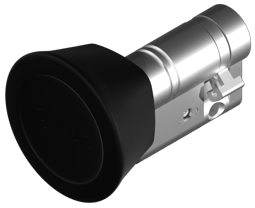
\includegraphics[scale=0.50]{img/europrofile-half-cylinder-D50S-121A-SD.png}
  \caption{Fechadura de meio cilindro \textit{Europrofile D50S.121A.SD} para o sistema iLOQ S50 \cite{iloq-lock}}
\end{figure}

\subsection{Código QR}

Um código QR é um tipo de código de barras bidimensional que permite guardar quantidades de dados muito maiores do que os típicos códigos de barras unidimensionais, e de forma muito mais fiável por utilizar um algoritmo de correção de erros. É essencialmente uma matriz de quadrados pretos ou brancos que codifica geralmente texto ou um URL, e possui várias características que lhe permitem ser lido em qualquer orientação e corrigir erros (tanto erros devidos à danificação do código como à qualidade da câmara). Um código QR pode ser recolhido usando uma câmara, e é depois processado usando um algoritmo de correção de erros de Reed-Solomon.

\begin{figure}[ht]
  \centering
  \includesvg[width = 37mm]{img/qr.svg}
  \caption{Um código QR deste tamanho pode guardar um identificador único de entre $4 \times 10^{9}$ combinações, e pode ser lido mesmo que 25\% da sua superfície esteja danificada.}
\end{figure}

Este tipo de código é amplamente utilizado, dada a quantidade significativa de informação que consegue guardar, a sua facilidade de criação e leitura (qualquer telemóvel consegue capturar um código e processá-lo), assim como o vasto número de implementações deste algoritmo sobre a forma de aplicações móveis.

\subsection{Pesagem de lixo a bordo}

A forma mais direta de quantificar os resíduos urbanos gerados pelas pessoas é a medição da sua massa. Por este motivo, as tecnologias de pesagem de lixo a bordo do camião têm vindo a crescer em popularidade por permitirem às entidades gestoras melhor determinar as rotas de recolha para reduzir os custos de operação da sua frota. Muitas entidades gestoras já utilizam este género de tecnologias, mas a maior parte não os anuncia por não ter grande utilidade às pessoas ou por uma certa percepção de monitorização exagerada dos hábitos de consumo.

A pesagem pode ser efetuada usando uma célula de carga com um extensómetro para medir a amplitude da deformação da célula de carga, que permite medir com grande precisão o peso de um determinado objeto de forma eletrónica. Um extensómetro é uma peça composta essencialmente por um fio em zigue-zague que, quando o seu comprimento é alterado na direção predominante do fio, provoca uma pequena alteração no comprimento do fio, e consequentemente na sua resistência elétrica, que pode ser medida de forma muito precisa.

\begin{figure}[ht]
  \centering
    \begin{subfigure}[b]{1.0\textwidth}
    \centering
    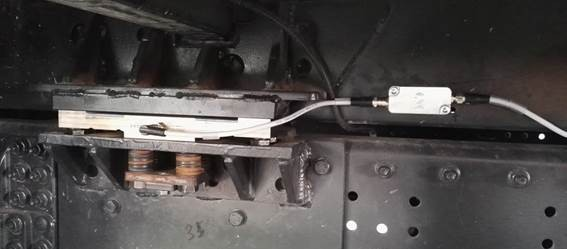
\includegraphics[height = 47mm]{img/distromel-chassis.jpg}
    \caption{No compartimento de carga, Distromel \cite{distromel-news}}
  \end{subfigure}
  
  \vspace{0.5em}
  
  \begin{subfigure}[b]{0.52\textwidth}
    \centering
    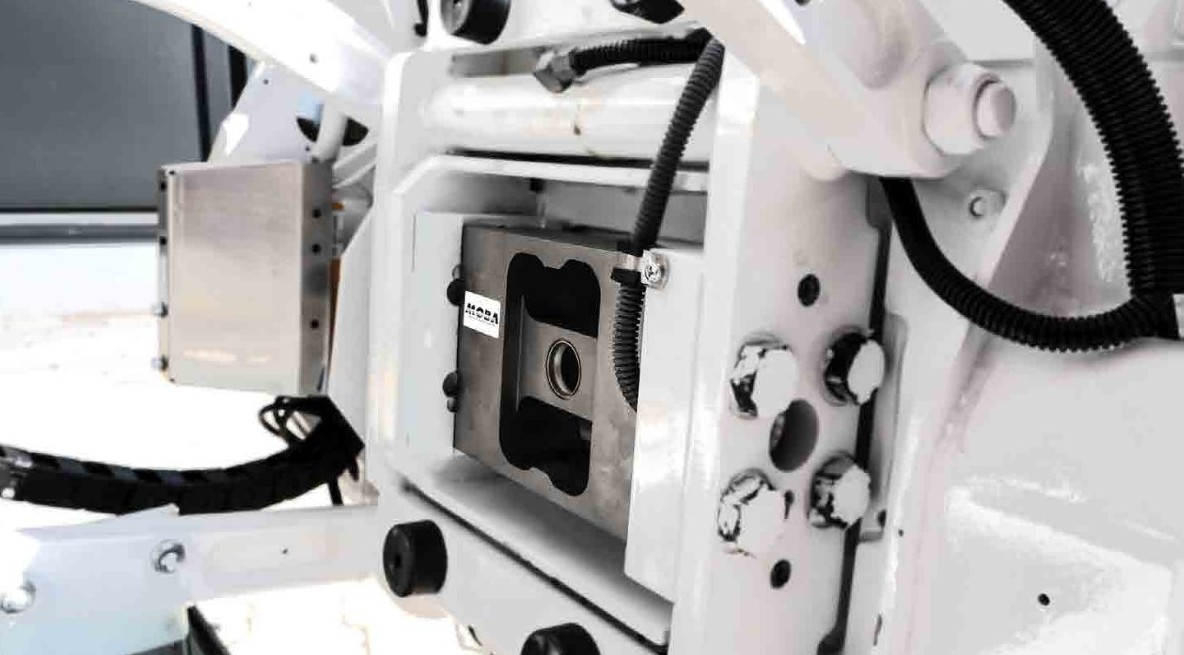
\includegraphics[height = 46mm]{img/moba-rear-elevator.jpg}
    \caption{No braço elevatório, MOBA \cite{moba-dynamic-scale}}
  \end{subfigure}
  \begin{subfigure}[b]{0.47\textwidth}
    \centering
    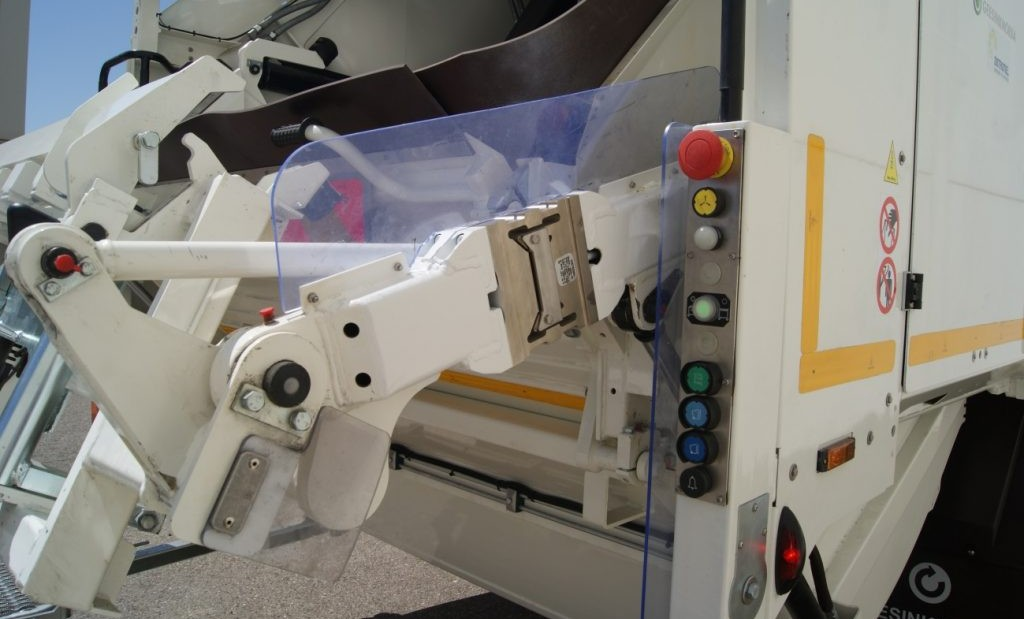
\includegraphics[height = 46mm]{img/distromel-rear-elevator.jpg}
    \caption{No braço elevatório, Distromel \cite{distromel-news}}
  \end{subfigure}
  \caption{Soluções com células de carga apresentadas por algumas empresas}
\end{figure}

Várias empresas fornecem soluções de pesagem de lixo a bordo de camiões, como a MOBA \cite{moba} e a ELTE \cite{elte-dynamic-weighing} (com soluções para carregamento frontal e traseiro), ou a espanhola Distromel \cite{distromel-generic, distromel-news} (pelo menos para carregamento traseiro).

Em muitos camiões de lixo este tipo de tecnologia já se encontra incluído, mas pode ser também facilmente adicionado a camiões que não a tenham. Estimamos (a partir dos preços de fábrica dos componentes e da mão-de-obra) que a instalação de um destes sistemas num camião de lixo custa entre \SIrange{100}{200}{\euro}, o que é incomparavelmente menor do que a escala de magnitude deste contexto, uma vez que um camião de lixo novo custa à volta de \SIrange{100000}{200000}{\euro}.

\subsection{Medidor de nível}

Na gestão inteligente de resíduos sólidos urbanos, é essencial saber, além do peso, quanto volume ainda se encontra vazio num contentor. Os chamados FLS (\textit{fill-level sensors}, sensores de nível de enchimento) permitem medir a distância entre a tampa e o lixo, sendo assim capazes de determinar quanto espaço ainda se encontra livre. Estes dispositivos são colocados no interior dos contentores, voltados para baixo, e usam sensores infravermelho ou ultrasons.

Estes dispositivos são especialmente desenhados para terem grande autonomia, durabilidade, resistência a impactos (comum no processo de recolha de resíduos) e às substâncias que possam ser libertadas pelos resíduos, de forma a adaptarem-se bem às condições de operação esperadas. Várias empresas fornecem este género de dispositivos, entre as quais a Distromel \cite{distromel-generic}, ELTE \cite{elte-fls} e MOBA \cite{moba-fls}. Alguns incluem ainda sensores de temperatura para detetar incêndios dentro dos contentores (vandalismo ou fogo acidental) e acelerómetros para detetar movimentações inesperadas (roubo do contentor, do lixo ou vandalismo).

\begin{figure}[ht]
  \centering
  \begin{subfigure}[b]{0.52\textwidth}
    \centering
    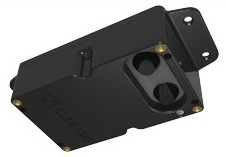
\includegraphics[height = 40mm]{img/elte-fls.jpg}
    \caption{ELTE Bin Box \cite{elte-fls}}
  \end{subfigure}
  \begin{subfigure}[b]{0.47\textwidth}
    \centering
    
\includegraphics[height = 40mm]{img/moba-fls.png}
    \caption{MOBA FLS \cite{moba-fls}}
  \end{subfigure}
  \caption{Sensores de nível de enchimento}
\end{figure}

\chapter{Descrição do projeto}
\label{ch:descricao}

A implementação deste projeto depende da satisfação de três grandes partes:

\begin{itemize}
    \itemsep0em
    \item Pré-acordo com as instituições (municípios, empresas de gestão de resíduos, ...)
    \item Desenvolvimento do equipamento necessário (pesagem de caixotes do lixo nos locais  onde há recolha ao domicílio, ou pesagem nos ecopontos).
    \item Desenvolvimento do software de gestão, da aplicação móvel/web app e do servidor que suporte ambas as interfaces.
\end{itemize}

Para efeitos de gestão de resíduos, considera-se que a menor unidade é a \textit{habitação}. Uma habitação é uma fração, edifício, conjunto de edifícios, terreno não-edificado ou outro, ao qual seja prestado o serviço de recolha de resíduos, mesmo que não seja habitado (a escolha da palavra \textit{habitação} deve-se principalmente à facilidade de compreensão do projeto). Cada habitação é identificada pelo seu endereço postal. De forma a simplificar a logística, vamos considerar que a cada contador de água corresponde uma habitação.

\section{Sistema centralizado}

A implementação deste projeto requer o desenvolvimento de um sistema centralizado para gerir e apresentar os dados resultantes da operação do sistema, e melhor planear como reagir a alterações no sistema.

Este sistema é desenvolvido apenas uma vez (por se tratar essencialmente de \textit{software}), e é distribuído a cada entidade gestora. Cada entidade gestora deve adquirir uma licença para usar o sistema, que deverá ser anual e custar uma quantidade não simbólica, mas bastante menor do que o custo inicial para a entidade gestora (que inclui também equipamentos, a parte mais cara).

O sistema irá receber informação regularmente de ecopontos, de forma a poder apresentar informação sobre a disponibilidade de cada ecoponto de receber mais resíduos. O sistema permitirá também centralizar a informação recolhida pelos camiões de lixo assim que terminem os serviços de recolha e regressem à base.

Este sistema será implementado como um servidor HTTP, de forma a ser o mais flexível possível; este servidor deve ser capaz de interagir também com a rede celular móvel, para receber a informação dos ecopontos. O sistema fornecerá uma API (\textit{application programming interface}) com autenticação, permitindo ser acedido por membros da entidade gestora através de um \textit{website} a partir de qualquer dispositivo que disponha de um \textit{web browser}. Esta API será também usada para permitir à aplicação móvel/web app utilizada pelos cidadãos aceder a alguma informação do sistema, principalmente a informação que lhes disser respeito.

\section{Recolha de resíduos}

Existem essencialmente três formas distintas de recolha de lixo:
\begin{itemize}
    \itemsep0em
    \item As pessoas que habitam em casas em zonas esparsamente povoadas beneficiam tendencialmente de recolha periódica ao domicílio.
    \item As pessoas que habitam em apartamentos fora de grandes centros populacionais ou em condomínios beneficiam de recolha periódica de contentores alocados ao condomínio ou ao prédio.
    \item As pessoas que habitam em grandes centros populacionais utilizam ecopontos, dado que a densidade populacional justifica uma grande densidade de ecopontos, que é suficiente para que a deslocação a um ecoponto não acarrete incómodo excessivo.
\end{itemize}

De forma a quantificar os resíduos urbanos gerados pelas pessoas, deve ser empregue o equipamento necessário à pesagem dos resíduos sólidos urbanos nestes três contextos.

\subsection{Recolha ao domicílio}
% explicitar melhor o "fornecer" / caso de vandalismo -> câmara fornece 1a unidade
A entidade gestora deve adquirir ao presente projeto vários caixotes do lixo de cada tipo de resíduo, munidos das seguintes tecnologias:
\begin{enumerate}
    \itemsep0em
    \item Uma etiqueta NFC passiva, que permite a leitura do identificador único do caixote (que se encontra associado a determinada habitação e ao tipo de lixo a que se destina) que permite a um dispositivo que use o sistema NFC facilmente identificar o caixote do lixo.
    \item Um código QR que contenha o mesmo identificador único do caixote, usado como alternativa à etiqueta NFC passiva se esta se encontrar danificada.
\end{enumerate}

A entidade gestora deve posteriormente fornecer às pessoas os caixotes dimensionados de acordo com as necessidades estimadas da habitação.

Adicionalmente, os camiões de recolha de lixo devem estar munidos das seguintes tecnologias:
\begin{enumerate}
    \itemsep0em
    \item Um leitor NFC, que permita ler a etiqueta NFC do caixote, de forma a identificar a habitação que será creditada com esse lixo.
    \item Uma balança, equipada no braço mecânico do camião, para medir a massa de lixo (basta subtrair a tara do caixote do lixo), ou equipada no compartimento do lixo (mede-se a diferença de massa antes e depois de esvaziar o caixote).
\end{enumerate}

\subsection{Recolha em ecopontos}

A entidade gestora deve equipar os seus ecopontos com as seguintes tecnologias:
\begin{enumerate}
    \itemsep0em
    \item Um dispositivo NFC ativo, que contém um identificador único desse contentor, e que controla uma tranca de forma a que, a cada vez que o contentor é aberto para depositar lixo, seja possível saber qual habitação será creditada com esse lixo.
    \item Uma balança, para medir a massa de lixo que cada pessoa colocou no ecoponto (as medições são realizadas a cada vez que o ecoponto é aberto).
    \item Um sensor de nível de enchimento, para permitir saber quanto volume do ecoponto se encontra vazio.
    \item Um chip com SIM integrado para comunicar periodicamente com o sistema informático centralizado através da rede celular.
\end{enumerate}

A pedido das pessoas, a entidade gestora também deve emitir cartões com etiquetas NFC passivas, de forma a que pessoas que não disponham de dispositivos móveis que suportem NFC ou que não se encontrem disponíveis possam continuar a depositar os seus resíduos.

\subsection{Recolha de contentores coletivos}

O caso em que várias habitações utilizam os mesmos contentores não acessíveis ao público (por exemplo, num prédio de apartamentos gerido por um condomínio e com casa de lixo) possui semelhanças com a recolha ao domicílio (os contentores são propriedade privada do condomínio e encontram-se geralmente guardados em casas de lixo) e em ecopontos (várias residências usam os mesmos contentores), pelo que é necessária uma abordagem mista.

A entidade gestora deve fornecer ao condomínio contentores de lixo equipados com a mesma tecnologia que os ecopontos, dispensando apenas o sensor de nível de enchimento e o chip com SIM dado que estes contentores não costumam estar disponíveis ao público e para os supostos utilizadores (os moradores desse condomínio) não é excessivamente incómodo deslocarem-se até à casa do lixo e verificarem se os contentores estão cheios.

\section{Aplicação móvel}

A aplicação móvel permite aos utilizadores acompanhar o processo de recolha e gestão dos resíduos que geraram. Cada utilizador deverá associar a aplicação à habitação que pretende gerir; cada utilizador pode associar mais que uma habitação à aplicação (para poder gerir várias habitações ao mesmo tempo), e vários utilizadores podem ter as suas aplicações associadas à mesma habitação (para, por exemplo, todos os residentes de uma habitação poderem acompanhar a gestão dos seus resíduos conjuntos).

A aplicação móvel atende a um conjunto de objetivos centrais, ao permitir às pessoas:
\begin{itemize}
    \itemsep0em
    \item Tomar consciência da quantidade de resíduos que geram, de certa forma responsabilizando-as.
    \item Saber que ecopontos ainda possuem espaço para evitar deslocações desnecessárias a ecopontos cheios de lixo.
    \item Serem avisados com antecedência sobre quando serão as próximas recolhas, no caso de usufruírem de recolhas periódicas de lixo ao domicílio, de forma a colocarem os caixotes/contentores do lixo em local adequado para a recolha.
    \item Pesquisar rapidamente em que contentor devem depositar um certo tipo de lixo.
\end{itemize}

Os mockups encontram-se disponíveis no anexo \ref{ch:anexo-mockups}.

\newpage

\section{Modo de operação}

Esta secção sumariza as anteriores, de forma a mostrar como os diferentes utilizadores podem interagir com este sistema.

\subsection{Para o cidadão}

O cidadão pode-se autenticar na aplicação de duas formas:
\begin{itemize}
    \itemsep0em
    \item Na aplicação móvel e web app, pode usar o identificador e palavra-chave enviados todos os meses na fatura de RSU. O identificador e palavra-chave são os mesmos todos os meses.
    \item Na aplicação móvel, pode usar o código QR no caixote do lixo (se for recolha ao domicílio) ou no cartão (nos outros casos) e a palavra-chave na fatura de RSU.
\end{itemize}

O cidadão pode usar o sistema das seguintes formas:

\begin{itemize}
    \item Se o cidadão usufruir de recolha ao domicílio, a entidade gestora distribui à sua residência ou estabelecimento caixotes/contentores de lixo dimensionados de acordo com as necessidades esperadas. O cidadão deve ainda colocar o caixote correto para recolha numa zona adequada (por exemplo, o passeio ou a beira da rua) no horário estabelecido para recolha (que pode ser regular ou ser dinâmico em função das necessidades esperadas através de recolhas de lixo anteriores).
    \item Se o cidadão usufruir de contentores coletivos, o condomínio disponibiliza contentores coletivos com tecnologias de pesagem como referido anteriormente, assim como também disponibiliza cartões de identificação aos seus condóminos. O cidadão deve separar o seu lixo dentro de portas, e posteriormente usar a aplicação móvel ou o cartão para se autenticar junto dos contentores coletivos, e depositar os resíduos separados nos respetivos contentores.
    \item Se o cidadão não usufruir de nenhum dos métodos anteriores, assume-se que dispõe de ecopontos das imediações da sua residência. O cidadão deve separar o seu lixo dentro de portas, e posteriormente usar a aplicação móvel ou o cartão para se autenticar junto dos ecopontos, e depositar os resíduos separados nos respetivos ecopontos.
\end{itemize}

Se o caixote se encontrar danificado, ou se os lixeiros detetarem o funcionamento errado do equipamento entregue ao cidadão, a entidade gestora deve ser contactada; sugere-se que a entidade gestora não cobre pelos caixotes entregues na primeira vez, mas que se o caixote se danificar que a entidade gestora cobre ao cidadão uma quantia igual à que a entidade gestora dispender para adquirir um caixote novo à nossa empresa.

\subsection{Para o condomínio}

Cada condomínio receberá um ou vários contentores coletivos de lixo, de todos os tipos de resíduos, que deverá disponibilizar aos condóminos. Além disso, cada condomínio deve informar a entidade gestora de quantas residências irão beneficiar do sistema, para a entidade gestora requisitar e entregar os respetivos cartões. O administrador do condomínio age sempre em nome dos condóminos, dado que se considera ser o responsável pela manutenção dos equipamentos e pela requisição à entidade gestora de cartões para os condóminos. O administrados do condomínio não pode cobrar qualquer valor sobre a utilização dos contentores coletivos, e apenas pode cobrar pelos cartões a mesma quantia que dispendeu para os adquirir à entidade gestora.

Da mesma forma que na recolha ao domicílio, o primeiro conjunto de contentores deve ser gratuíto para o condomínio, e sugere-se que a danificação de um contentor leve a entidade gestora a fornecer um novo contentor ao condomínio pelo mesmo valor que pagou à nossa empresa por esse contentor.

\subsection{Para o pessoal de recolha de lixo}

Os coletores de lixo (também conhecidos como \textit{lixeiros}) não necessitam de alterar significativamente a sua atuação, exceto em dois aspetos:

\begin{itemize}
    \item Na recolha domiciliária, devem abrir os caixotes para analisar rapidamente e decidir, dentro da razoabilidade e do curto intervalo de tempo disponível, se os resíduos se encontram suficientemente bem separados; se não se encontrarem corretamente separados a recolha não deve ser realizada.
    \item Na recolha de contentores coletivos, devem abrir os contentores para analisar rapidamente se os resíduos se encontram suficientemente bem separados; se não for o caso, devem recolher o lixo na mesma mas tomar nota dessa ocorrência.
\end{itemize}

O condutor do camião do lixo é também responsável por monitorizar o correto funcionamento e utilização dos equipamentos durante um serviço de recolha, assegurando-se que os caixotes são corretamente identificados pelo sistema a bordo e que a massa de lixo é avaliada. Além disso, assim que terminar um serviço, o condutor do camião do lixo deve introduzir a informação no sistema; a operação deverá ser simples, bastando aproximar um dispositivo para realizar leitura por NFC ou usando um microchip com memória \textit{flash}.

\subsection{Para o gestor}

A entidade gestora é responsável pelo correto funcionamento dos equipamentos em geral, devendo assegurar-se que os equipamentos a bordo dos camiões se encontram em funcionamento, e suportar as despesas que advierem da necessidade de os reparar/substituir. Além disso, a entidade gestora também é diretamente responsável pelo correto funcionamento do equipamento dos ecopontos.

Um administrador do sistema (geralmente um membro da entidade gestora com permissões elevadas) consegue aceder a toda a informação no sistema. A entidade gestora é responsável pelo uso cuidadoso da informação que dispõe; a empresa que implementa este projeto fornece os meios tecnológicos para assegurar a privacidade e segurança dos dados dos munícipes e utilizadores, mas os membros da entidade gestora são em última análise os encarregados de utilizar esses dados de forma responsável.

\section{Estudo da concorrência}

Várias empresas fornecem soluções semelhantes à presente proposta, com abrangências diferentes, níveis distintos de monitorização, e objetivos diferentes. Não obstante, a maior parte das soluções foca-se excessivamente na otimização da entidade gestora e gestão de frota (localização GPS dos veículos e contentores, monitorização de contentores, gestão de combustível, ...) e não na justiça ambiental, ou não são suficientemente justas por não serem abrangentes ou por não determinarem de forma justa a produção estimada de lixo.

Vários projetos semelhantes encontram-se em implementação/planeamento ou já se encontram implementados em Portugal, mas possuem vários problemas associados. O mais comum (e que se encontra presente em todos os projetos que analisámos em Portugal) é que apenas os resíduos indiferenciados são tributados e os restantes resíduos recicláveis (plástico/metal, papel, vidro) não são contabilizados; este sistema incentiva as pessoas a apenas produzir menos resíduos indiferenciados, mas não promove a redução do total de resíduos gerados, que é uma meta muito importante porque os resíduos "recicláveis" não podem ser reciclados indefinidamente, pelo que uma parte desses resíduos terá que ser tratado de outra forma (geralmente enviados para aterros ou descarregados para o mar, com grande impacto ambiental).

Além disso, ao considerar-se apenas os resíduos indiferenciados, os restantes resíduos são completamente ignorados, quando se pode tomar como certo um dos seguintes cenários:

\begin{enumerate}
    \itemsep0em
    \item Ou estes resíduos têm tanto valor que podem mais tarde ser vendidos a um valor superior àquele que custou efetuar a recolha e processamento, sendo que os munícipes deviam ser recompensados.
    \item Ou estes resíduos não têm valor suficiente, e os munícipes devem continuar a pagar para a entidade gestora processar esses resíduos, se bem que uma quantia menor dado que esses resíduos são valorizados.
\end{enumerate}

O que não se pode é tentar convencer as pessoas de que o processamento e valorização destes resíduos é uma operação com resultado financeiro nulo.

\subsection{Tara recuperável}

Os projetos de tara recuperável consistem na atribuição de um valor monetário (ou pontos num certo sistema, que se podem traduzir em benefícios) quando uma pessoa deposita um certo tipo de resíduos num contentor de recolha seletiva desse resíduo. Por exemplo, a devolução de garrafas de vidro de leite ou cerveja de tamanhos padronizados constituem os sistemas mais antigos de tara recuperável, por ser um tipo de embalagem muito utilizada e que, depois de limpa, apenas precisam de ser enchidas (e rotuladas de novo, se necessário), seladas e enviadas para superfícies comerciais. É possível efetuar também este procedimento para outros resíduos, nomeadamente embalagens de plástico PET, apesar do processo de recuperação de garrafas PET ser geralmente mais complexo por ser necessário criar embalagens de tamanhos diferentes (reciclagem), que difere do sistema de tara recuperável de embalagens de vidro padronizadas (que na prática constitui reutilização e não reciclagem).

Os projetos de tara recuperável possuem todos o mesmo tipo de problemas: por serem de caráter voluntário não permitem implementar o princípio do poluidor-pagador e assim atingir uma justiça ambiental mais eficaz; além disso, este tipo de sistemas não pretende ser inclusivo, ao contrário da nossa proposta que permite, de forma obrigatória, gerir todos os resíduos de todas as pessoas de uma forma integrada com o funcionamento normal das entidades gestoras de resíduos e que não interfere exageradamente com as rotinas das pessoas.

\subsection{ELTE}

O grupo ELTE está cediado em Manchester (Inglaterra) com subsidiárias na Alemanha e Polónia. Este grupo de empresas fornece essencialmente soluções para gestão de frotas e recolha de lixo, com clientes em quase todos os países europeus, e foi contratada para implementar os serviços integrados de recolha de resíduos das cidades de Vilnius (Lituânia), Varsóvia (Polónia), Liubliana (Eslovénia) e Sófia (Bulgária).

Esta empresa foca-se principalmente em planeamento de rotas e gestão da frota, apesar de também disponibilizar soluções interessantes para medição do nível de enchimento dos contentores e pesagem a bordo. No entanto, o foco é marcadamente a gestão do processo de recolha de resíduos, dado que não são identificadas as pessoas que depositam o lixo em contentores coletivos.

\subsection{Distromel}

A Distromel é uma empresa espanhola, de Huesca (Aragão), de sistemas de controlo e medição nas áreas da industria, agricultura, logística e ambiente.

A solução apresentada pela Distromel, chamada SmartDTD, permite a implementação do sistema de poluidor-pagador em locais em que apenas é efetuada recolha ao domicílio. Na solução apresentada, cada caixote do lixo ou contentor possui uma célula de carga, e no momento de recolha do lixo apenas é necessário consultar a informação que o caixote/contentor tiver, dado que é o próprio caixote a efetuar a pesagem.

Esta solução é relativamente inovadora, mas comporta um conjunto de problemas que não podem ser ignorados e que tornam a solução demasiado complexa e difícil de implementar, e com muitos pontos de falha que podem comprometer o correto funcionamento do sistema:

\begin{enumerate}
    \item Cada caixote tem que ter uma célula de carga, que, dependendo da carga a que se destina, custa cerca de $\SI{30}{\euro/unidade}$ a preço de fábrica, o que aumenta o custo de um caixote do lixo de $\SI{100}{\liter}$ para mais do dobro (sem contar com o \textit{chip} que efetua as leituras).
    \item Cada caixote do lixo, mesmo os mais pequenos, deve ter uma bateria, o que dá origem a vários problemas:
    \begin{enumerate}
        \item Utilização excessiva de baterias com impacto ambiental correspondente;
        \item Necessidade de carregamento/substituição; a empresa refere que as baterias podem ser carregadas pelo camião do lixo, o que se antecipa bastante complicado porque as alternativas não se apresentam como particularmente interessantes:
        \begin{enumerate}
            \item O camião fazer uma ligação elétrica física à bateria, o que é inviável dadas as condições duras de utilização dos caixotes, que podem danificar os interfaces, assim como a dificuldade de alinhar interfaces elétricos num processo que se deseja o mais rápido possível para sujeitar os lixeiros ao menor tempo possível na rua (quase sempre desabrigados) e em contacto com o lixo. 
            \item Realizar o carregamento por indução eletromagnética, que se sabe ser relativamente demoroso no caso de baterias, dado que (a título de exemplo) uma pilha de relógio fornece $\SI{35}{\milli \ampere \hour}$ de carga a $\SI{1.55}{\volt}$, o que equivale a $\SI{0.05425}{\watt \hour} = \SI{195.3}{\joule}$ de energia, e os mais avançados carregadores de telemóveis sem fios conseguem fornecer até $\SI{10}{\watt}$, o que implicava pelo menos $\SI{20}{\second}$ para carregar a bateria. Tudo isto assumindo que a bateria é recarregável e que suporta ser carregada a $\SI{10}{\watt}$ (os carregadores de pilhas domésticos costumam carregar pilhas AA a $\SI{600}{\milli \ampere}$, o que equivale a cerca de $\SI{0.9}{\watt}$ para uma pilha AA de $\SI{1.5}{\volt}$), e que o \textit{chip} no caixote não é danificado por um campo eletromagnético tão forte.
        \end{enumerate}
    \item Nenhuma desta tecnologia dispensa mesmo assim a instalação de dispositivos adicionais nos camiões, incluindo células de carga no braço elevador ou no compartimento de carga.
    \end{enumerate}
\end{enumerate}

\subsection{MOBA}

A Mobile Automation (MOBA) é uma empresa alemã de tecnologia para maquinaria pesada em indústria, cediada em Limburg an der Lahn, Hesse. A MOBA possui 14 subsidiárias e tem presença em 13 países da América, Europa e Ásia/Oceânia, assim como dezenas de revendedores, incluindo em Portugal.

A MOBA fornece soluções principalmente nas áreas da construção de estradas, movimentação de terra, gruas e gestão de resíduos, sendo esta última a que nos importa. Nessa área, são oferecidos produtos de pesagem móvel, identificação via rádio e medição de nível de enchimento de contentores, e serviços de gestão de rotas e armazenamento na nuvem. Esta empresa fornece portanto um sistema integrado de gestão de resíduos, tratando-se essencialmente disso: um sistema de gestão de resíduos. Esse foco excessivo na entidade gestora é positivo para a própria entidade, mas torna difícil para os cidadãos compreender os ganhos subjacentes, além da ênfase numa abordagem punitiva (poluidor-pagador) aparentemente apoiada na ideia de que os contentores do lixo recolhem todo o tipo de lixo sem separação, em vez de promover a redução do lixo gerado em primeiro lugar, a separação e reciclagem do lixo, e o retorno financeiro para os cidadãos.

\subsection{Projeto Orgânico (Porto)}

O Projeto Orgânico é um projeto do município do Porto (operacionalizado pela Porto Ambiente) com o objetivo de promover a separação de resíduos orgânicos em casa \cite{organico-home}. Este projeto foi lançado a 22 de abril de 2021, abrangendo cerca de 60\% dos habitantes da cidade do Porto \cite{organico-news}, e consiste na distribuição voluntária de baldes de lixo de $\SI{5}{\liter}$ a cada residência, que devem ser usados para separação dos resíduos orgânicos em casa; o balde deve ser posteriormente despejado pelo residente num contentor especial para resíduos orgânicos num ecoponto, usando um cartão para se identificar e abrir o contentor.

Este projeto é um bom ponto de partida e avança uma ideia interessante: considerar um novo tipo de resíduos, os orgânicos, que podem ser muito facilmente aproveitados como composto orgânico se forem corretamente separados do lixo indiferenciado (o que implica que não podem ser colocados no contentor de resíduos orgânicos sacos de lixo de plástico contendo resíduos orgânicos dado que o plástico polui o composto, logo o balde do lixo deve ser transportado desde a residência até ao ecoponto e ser diretamente despejado para o contentor).

No entanto, existem alguns problemas e omissões:

\begin{enumerate}
    
    \item Não pode ser contabilizada a produção de lixo orgânico para distribuição de incentivos, dado que, apesar de ser necessário um cartão para abrir um contentor de lixo orgânico, não é indicada a presença de algum método de medição da quantidade de resíduos depositados por cada indivíduo nesse contentor, nem é possível extrapolar que residências/estabelecimentos utilizam esse contentor (até porque cada pessoa que pretenda depositar resíduos orgânicos pode fazê-lo num contentor qualquer), nem sequer tentar alterar a taxa de resíduos para todos os residentes e estabelecimentos nessa zona dado que se espera, por exemplo, que estabelecimentos de restauração produzam uma quantidade muito maior de resíduos orgânicos do que uma residência.

    \item As pessoas não podem receber incentivos, dado que não é possível contabilizar a produção de lixo orgânico; o único incentivo é o de saberem (se sequer souberem ou quiserem saber) que a empresa municipal de gestão de resíduos será capaz de produzir um composto orgânico que produz receitas dos quais os residentes nunca beneficiarão diretamente, se é que alguma vez beneficiarão.
    
    \item A ausência de incentivo nem punição para contribuir para a separação correta dos resíduos orgânicos compromete a qualidade do composto orgânico a ser produzido, dada a seguinte análise empírica e simples sobre o comportamento das pessoas:
    \begin{enumerate}
        \item Se os outros contentores estiverem cheios, há um impulso para as pessoas depositarem os resíduos nos locais incorretos. Se os contentores de plástico, vidro, papel ou orgânicos estiverem cheios, as pessoas costumam depositar os resíduos no contentor do lixo indiferenciado; mas se este contentor estiver cheio, é fácil de imaginar que as pessoas depositem os resíduos no contentor que parece mais adequado, que deverá ser o de resíduos orgânicos por ser mais parecido com o de resíduos indiferenciados à primeira vista.
        \item Por hábito ou por facilidade de transporte, alguns residentes continuarão a usar sacos de plástico para transportar resíduos orgânicos; é muito comum cobrir o interior do balde para evitar lavar o balde do lixo tão frequentemente, apesar da indicação de que os baldes são facilmente laváveis numa máquina de lavar a loiça e que devem ser diretamente despejados para o contentor respetivo.
    \end{enumerate}
\end{enumerate}

\subsection{Recicle Mais, Pague Menos (Maia)}

Em 2012, o município da Maia, através da empresa municipal de gestão de resíduos Maiambiente, e em conjunto com a LIPOR, começou a implementar o projeto "Ecoponto em Casa", com a distribuição de caixotes de lixo com identificadores eletrónicos a quase todas as residências individuais do município \cite{ecopontoemcasa-primeiramao, rmpm-noticiasmaia, rmpm-primeiramao}. Este projeto recebeu grande atenção de outros municípios vizinhos, em Portugal e mesmo na União Europeia \cite{rm-ue}.

Em 3 de maio de 2021, a Câmara Municipal da Maia deu início ao projeto "Recicle Mais, Pague Menos" (R+P-), que, apoiado no projeto anterior, possibilitará a implementação do princípio do poluidor-pagador, que, ao fim das três fases, irá a partir de 2024 contribuir para o cálculo da taxa de resíduos sólidos urbanos para cada residência individual em função do número de vezes que os caixotes são esvaziados pelos camiões de lixo \cite{rmpm-primeiramao}, assumindo-se que a recolha de outros resíduos é gratuíta.

Este é o primeiro projeto de \textit{pay-as-you-throw} em larga escala em Portugal, mas não sem alguns problemas óbvios:

\begin{enumerate}
    \item Contempla apenas recolha ao domicílio, ignorando residentes de apartamentos ou condomínios em grandes centros e ecopontos.

    \item A contabilização dos resíduos gerados pelo número de recolhas de resíduos indiferenciados não é justa, pois alguns resíduos possuem a mesma massa (logo, possuem a mesma quantidade de matéria-prima revalorizável) mas diferentes volumes, sendo que dois caixotes com o mesmo volume de resíduos de diferentes densidades são tributados da mesma forma apesar de um deles poder ter resíduos mais densos, e logo com mais valor. Assim, nem sequer faz sentido tentar estimar o peso em lixo que um caixote de lixo indiferenciado cheio contém.
    \item São promovidos hábitos pouco saudáveis, como:
    \begin{enumerate}
        \item A acumulação de resíduos durante longos períodos no caso de residências onde são produzidos poucos recursos, sendo pouco higiénico manter lixo durante muito tempo dentro de casa, mesmo que em pequenas quantidades.
        \item Um esforço de comprimir os resíduos de forma a caber maior quantidade no mesmo caixote, o que pode provocar dificuldade a esvaziar o caixote por os resíduos estarem comprimidos e endurecidos (ficam "colados" ao caixote) e a movimentar um caixote pesado.
    \end{enumerate}
\end{enumerate}

\subsection{PAYT (Guimarães)}

Em abril de 2016, a VITRUS iniciou a implementação de um projeto PAYT no centro histórico da cidade de Guimarães, abrangendo cerca de 1500 pessoas. Este projeto consiste na distribuição de sacos de lixo de plástico certificados pela VITRUS com capacidades de $\SI{15}{\liter}$, $\SI{30}{\liter}$, $\SI{50}{\liter}$ e $\SI{100}{\liter}$, e só são recolhidos resíduos indiferenciados nessa zona da cidade se estiverem dentro destes sacos certificados. Isto significa que as pessoas pagam pelo lixo que produzem quando compram os sacos, dado que apenas são recolhidos os sacos certificados e vendidos pela VITRUS \cite{guimaraes-payt}. Os restantes resíduos são recolhidos gratuitamente.

Este projeto padece de alguns dos problemas do sistema a ser implementado na Maia; nomeadamente, partilha do problema de não serem contabilizados os outros resíduos, e do volume dos resíduos indiferenciados. Além disso, possui vários problemas adicionais relacionados com os sacos de lixo:

\begin{enumerate}
    \item Ao exigir que se usem sacos plásticos para conter os resíduos indiferenciados, está-se a promover o consumo regular de plásticos de utilização única;
    \item O problema de promoção de hábitos que comprometem a saúde pública no caso da Maia também se extende a este projeto, dado que a utilização de sacos em vez de caixotes do lixo pode contribuir para uma perceção pública de que apenas é necessário sacos de lixo para conter os resíduos indiferenciados e levar as pessoas a dispensar de usar caixotes de lixo, levando ao amontoamento de sacos de lixo na rua em vez de estarem adequadamente guardados num caixote/contentor (mesmo que o projeto indique que só se deve colocar os sacos na rua $\SI{10}{\minute}$ antes da recolha, é óbvio que nem toda a gente vai fazer isso, e vão simplesmente colocar os sacos na rua assim que ficarem cheios para evitar que ocupem espaço dentro da residência/estabelecimento e que libertem maus odores em espaços fechados), o que pode ter consequências em dois aspetos:
    \begin{itemize}
        \item Afetar a perceção de higiene pública;
        \item Ao estarem mais expostos a condições climatéricas e à natureza, os sacos podem romper e libertar odores e líquidos escorridos, assim como dar origem a roubo de lixo e a atração de animais que se alimentem deste tipo de resíduos (ratos, gaivotas, etc.).
    \end{itemize}
    \item O facto de o pagamento ser feito por saco significa que as pessoas se sentem incentivadas a apenas livrarem-se deles quando estiverem cheios, o que origina mais uma vez o problema de acumulação de resíduos indiferenciados nas residências durante longos períodos.
    \item Além disso, as pessoas tentam assim colocar a maior quantidade de resíduos indiferenciados possível no mesmo saco, ultrapassando os limites estabelecidos para esses sacos, aumentando a dificuldade de manuseamento para os lixeiros e a probabilidade de rotura durante o manuseamento ou enquanto aguardam recolha.
\end{enumerate}

\newpage

\section{Análise SWOT}

Apresenta-se a seguir a análise SWOT deste projeto, de forma a sumariamente descrever os fatores internos mais importantes a ter em conta durante a sua implementação, e o ambiente em que este projeto atuará.

\begin{center}
    \begin{tabular}{c l @{}}
        \cellcolor{strengthgreen!80 }\color{white}{\Large\textbf{Strengths}} &
            \begin{minipage}{122mm}\vspace{0.4em}\begin{itemize}\itemsep0em
                \item O sistema que propomos é abrangente, ou seja, prevê soluções para todas as situações de recolha de resíduos e todos os casos de uso
                \item A contabilização dos resíduos gerados é justa.
                \item A solução proposta é tão complexa e dispendiosa quanto estritamente necessário.
            \end{itemize}\vspace{0.0em}\end{minipage} \\
        \cellcolor{red!80   }\color{white}{\Large\textbf{Weaknesses}} & 
            \begin{minipage}{122mm}\vspace{0.4em}\begin{itemize}\itemsep0em
                \item Grande financiamento à cabeça para desenvolver a aplicação móvel/web app e para a encomenda inicial e adaptação de caixotes do lixo.
                \item No início a empresa que implemente este projeto terá pouca liquidez, mas os valores das transações serão muito grandes (encomenda de caixotes por grosso, instalação do sistema, etc.). Uma empresa com receitas e despesas de ordens de magnitude muito superiores à sua liquidez (mesmo que equilibradas no instante presente) possui grande risco de desequilíbrio orçamental com pequenas alterações nas receitas ou despesas.
            \end{itemize}\vspace{0.0em}\end{minipage} \\
        \cellcolor{blue!80  }\color{white}{\Large\textbf{Opportunities}} &
            \begin{minipage}{122mm}\vspace{0.4em}\begin{itemize}\itemsep0em
                \item Maior consciência ambiental das pessoas.
                \item Vontade da sociedade e dos decisores políticos de promoção de uma economia ecológica, sustentável e amiga do ambiente.
                \item Legislação que fornece enquadramento legal e orientações relativas à implementação de sistemas inteligentes de gestão de resíduos urbanos que apliquem o princípio do poluidor-pagador.
                \item Financiamento nacional e europeu através de fundos nacionais e europeus, especialmente dado o atual contexto de promoção do investimento numa fase de recuperação económica pós-pandemia COVID-19.
            \end{itemize}\vspace{0.0em}\end{minipage} \\
        \cellcolor{orange!80}\color{white}{\Large\textbf{Threats}} &
            \begin{minipage}{122mm}\vspace{0.4em}\begin{itemize}\itemsep0em
                \item Problemas com atrasos no fornecimento (que se traduz em pagamentos efetuados por bens que a empresa ainda não possui fisicamente, com perda de liquidez sem bens para transacionar) dada a recessão económica e a quebra das cadeias de fornecimento provocada pela pandemia COVID-19.
                \item Atrasos nos pagamentos por parte das entidades gestoras, não só pelos motivos habituais mas também pelo desvio de fundos para outras medidas devido ao atual contexto económico (por exemplo, uma câmara municipal pode contratualizar um serviço a esta empresa, e decidir entretanto reduzir os fundos para essa contratualização para os mover para apoio emergencial a empresas municipais ou ao tecido empresarial do município).
            \end{itemize}\vspace{0.0em}\end{minipage}
    \end{tabular}
\end{center}

\chapter{Modelo de negócio}

\section{Análise de custos}

Os recursos a nível material, financeiro e humano necessários serão alvo de avaliação contínua, uma vez que estão diretamente relacionados com a escala a que o projeto se encontra. Contudo, haverá elementos que, embora possam variar em termos da sua relevância, serão uma constante a ter em conta.

De uma perspetiva mais geral consideramos que um espaço físico amplo de trabalho traria mais desvantagens (na forma de custos monetários) do que vantagens, pelo que achamos que a melhor opção seria um pequeno escritório com a função principal de residência fiscal, o que representa um encargo de $\SI{500}{\euro}$/mês.
Para além disto, a nível dos recursos humanos que estejam ligados à empresa e não diretamente ao serviço/produto que oferecemos, apenas esperamos que seja relevante a contratação de um serviço de avença com um escritório de advogados que nos garanta acompanhamento jurídico, o que acarreta um custo de aproximadamente $\SI{250}{\euro}$/mês e uma avença contabilística (um extra correspondente a mais $\SI{250}{\euro}$/mês). Eventuais processos a tratar em tribunal poderão implicar, previsivelmente, uma despesa adicional com custas judiciais no valor de $\SI{1000}{\euro}$/ano.

No que diz respeito ao produto em concreto, mais especificamente à aplicação web, a nível físico existe a necessidade de um servidor (\textit{server}) com um sistema centralizado instalado para garantir o acesso permanente (24h/dia e 365 dias/ano) à web app, guardando e mantendo disponível a informação disponível aos seus utilizadores - de que é exemplo a quantidade de lixo depositado, as pessoas associadas a cada habitação, e a próxima data de recolha (se aplicável). Este servidor com o sistema centralizado seria fornecido à entidade gestora (o que representaria um custo próximo dos \SIrange{2000}{3000}{\euro} cada), ou, em alternativa, se esta já possuísse um dispositivo capaz, este seria configurado devidamente, existindo neste último caso menos garantias relacionadas com a fiabilidade do mesmo.

Em relação à aplicação/sistema centralizado em si, esta implica custos fixos. Idealizamos uma aplicação de complexidade média-baixa, com uma interface polida, sistema de registo e login, domínio customizado, dashboard (painel de controlo), activity feed, integração de geolocalização com mapa incorporado, páginas de análise do tráfego, performance e falhas que eventualmente ocorram. Um ponto de foco é também a vertente da segurança de utilização recorrendo-se a um certificado SSL (que permite uma conexão encriptada entre a aplicação e o servidor web) e proteção contra outro tipo de ataques, de que são exemplo os ataques de negação de serviço, mais conhecidos por Denial-of-Service (DoS). Uma estimativa do desenvolvimento desta aplicação/sistema centralizado seria à volta dos $\SI{27000}{\euro}$ tendo a duração de 12 semanas, para uma equipa de 5 desenvolvedores de \textit{software} e de um desenvolvedor de UI/UX (interface/experiência do utilizador). Uma vez que o grupo de trabalho é da área da engenharia informática, apenas seria necessário procurar um designer. Em termos monetários, estamos a falar de $\SI{1400}{\euro}$/mês para cada um dos developers, a que acresce um valor que ronda os $\SI{1300}{\euro}$/mês para o designer durante as 12 semanas de desenvolvimento, existindo a possibilidade de, em caso necessidade, estender a existência desta última posição até um futuro mais distante. Os encargos destinados aos desenvolvedores diminuirão ao longo do tempo em resultado da diminuição da carga de trabalho (que eventualmente se resumirá à manutenção da aplicação), fixando-se nos $\SI{400}{\euro}$/mês.

Com a aplicação pronta torna-se necessário colocá-la accessível ao público. Uma possibilidade que não acarreta custos extra será disponibilizar o ficheiro APK no domínio web do projeto, podendo o utilizador descarregar para o seu telemóvel a aplicação. Contudo, este meio não é o mais eficaz para alcançar uma vasta parte da população, sendo necessário para o efeito o pagamento das devidas taxas às duas grandes empresas que possuem o monopólio de distribuição de aplicações móveis: Google e Apple. No caso da primeira, para ser possível colocar uma aplicação na Google Play Store é obrigatório o pagamento de uma taxa única de 25 dólares aquando de criação de uma conta Google Play Developer. Por sua vez, a Apple exige um pagamento anual de 99 dólares para permanecer no Apple Developer Program, ou seja, ter o direito de poder colocar a aplicação na loja online.

Voltando a atenção para os cartões alternativos à aplicação e para os caixotes do lixo a serem distribuídos pelos cidadãos, estes teriam a intervenção de empresas subcontratadas por nós. Em primeiro lugar, a produção de cartões corresponde a perto de $\SI{1}{\euro}$/cartão, variando bastante o preço da unidade consoante o tamanho da encomenda. Em segundo, para a produção de caixotes com os requisitos necessários, ou seja, um para cada tipo de lixo da respetiva cor e com uma etiqueta rádio identificadora do próprio caixote, a matéria-prima escolhida será um plástico do tipo HDPE (\textit{High-Density Popyethylene}), devido à sua resistência a variações de temperatura, impactos e substâncias químicas, características de grande relevo num produto deste género. O preço de mercado deste recurso encontra-se perto dos $\SI{0.85}{\euro/\kilogram}$ pelo que, tendo como modelo um peso médio de $\SI{5}{\kilogram}$ para cada caixote doméstico, uma estimativa plausível seria um custo de $\SI{4.25}{\euro}$ por caixote ao qual acrescia o valor da etiqueta NFC que é $\SI{0.25}{\euro}$.
Tendo em conta a logística necessária para a produção e posterior distribuição acreditamos que as despesas finais seriam na ordem dos $\SI{15}{\euro/caixote}$ (ou seja, $\SI{60}{\euro}$ assumindo o conjunto dos quatro tipos de lixo: papel, plástico, vidro, orgânico), podendo este valor por unidade vir a descer mediante a dimensão das encomendas.
Em relação aos contentores, uma célula de carga ronda os $\SI{125}{\euro}$ pelo que um custo plausível de atualização de um contentor seria perto dos $\SI{150}{\euro}$.

\section{Análise de rendimentos}

De forma resumida, no que toca aos rendimentos, estes estão divididos essencialmente em dois conjuntos: únicos e periódicos/passivos. No grupo das receitas únicas incluem-se a venda de caixotes e possível financiamento de fundos nacionais e/ou europeus. Por sua vez, as receitas resultantes de taxas paga pelas câmaras (periodicamente), correspondem aos rendimentos passivos.

Adquiridos entre \SIrange{10}{15}{\euro} por unidade (dependendo da escala da encomenda), os caixotes serão fornecidos aos municípios a $\SI{20}{\euro}$ a unidade, constituindo esta a principal fonte de rendimento, assumindo um cenário não tão otimista em que uma candidatura para programas de financiamento (de que foi exemplo o programa PO SEUR -- Programa Operacional para a Sustentabilidade e Eficiente Uso dos Recursos 2014-2020) seja rejeitada. Caso uma eventual candidatura a um projeto similar seja aprovada, estima-se uma verba de capital entre os \SIrange{50000}{100000}{\euro} que cobririam em grande maioria os encargos associados ao primeiro ano de operação, acelerando significativamente a chegada ao chamado \textit{break even point}, a partir do qual os custos deixam de exceder as receitas.
O pagamento anual da licença por parte de cada entidade gestora (município) para uso do sistema centralizado no valor de $\SI{5000}{\euro}$ anuais a que acresce uma taxa de $\SI{1}{\euro}$ por cada caixote que se encontrasse no terreno corresponde a uma fluxo monetário com grande potencial de crescimento que viabiliza a sustentabilidade do negócio a longo prazo.

\section{Análise de lucros}

O balanço final previsto para cada ano e com especial destaque para o primeiro é um ponto com bastantes 'se's . Um primeiro ano positivo resultante de um conseguido financiamento, não implica que dois anos depois já terá sido alçando o \textit{break even point}, apesar de ser um aspeto promissor para que aconteça. Não nos podemos esquecer de que o futuro é um mar de incertezas, mesmo que pensemos que o conseguimos prever com base em situações idênticas que tenham ocorrido no passado. Por esta razão, decidimos considerar 3 diferentes cenários.

Num primeiro cenário - considerado otimista - conseguir-se-ia um financiamento de $\SI{100 000}{\euro}$, o que permitiria terminar o primeiro ano de uma forma neutra em termos financeiros, já tendo em "atividade" uma amostra de 1000 caixotes que funcionariam como uma forma de uma câmara testar concretamente o impacto do projeto no terreno. O segundo traria prejuízos estimados de $\SI{26000}{\euro}$, mas o número de unidades distribuídas estaria na casa dos $\SI{5000}{\euro}$ em resultado de uma fase de testagem bem sucedida, sendo o \textit{break even point} alcançado, e logo no ano seguinte atingir-se-ia pela primeira vez um balanço anual positivo com números a rondar os $\SI{35000}{\euro}$ de lucro ou \SIrange{15000}{20000}{\euro} se tivermos em conta o acumulado dos anos anteriores. Nos anos seguintes continuar-se-ia a aumentar o número de caixotes em utilização e no quinto ano, as previsões apontam para que as taxas pagas pelo(s) município(s) sejam já suficientes para suportar os custos anuais, ou seja, se ocorresse algum percalço e não fossem vendidas mais unidades, continuaria a ser sustentável.
Voltando-nos agora para um cenário mais neutro, no qual o financiamento é igualmente conseguido mas num valor correspondente à metade do anteriormente referido (i.e. $\SI{50000}{\euro}$ em vez de $\SI{100000}{\euro}$) e o número de caixotes que é vendido é ligeiramente inferior em cada ano, resultante de limitações de produção, o lucro acumulado só viria a corresponder a um valor positivo durante o quarto ano de operações.
Por último, um cenário mais pessimista que os anteriores, no qual não é conseguido financiamento e o número de caixotes que é vendido é bastante inferior em resultado, por exemplo, de uma densidade populacional baixa das regiões aderentes e de problemas na linha de produção de caixotes, sugere uma estimativa em que o retorno do investimento chega apenas durante o quinto ano, ou seja, bastante atrasado comparado com os outros cenários apresentados.

Consultar gráficos no anexo \ref{ch:anexo-custos}.

\chapter{Plano de ação}

O desenvolvimento do projeto apresentado está divido nas seguintes fases:

\begin{enumerate}
    \itemsep0em
    \item Formação da equipa;
    \item Desenvolvimento do protótipo da app;
    \item Reuniões com fornecedores;
    \item Reuniões com as câmaras para apresentação do projeto;
    \item Obtenção de financiamento;
    \item Desenvolvimento da aplicação e produção dos caixotes;
    \item Marketing;   
    \item Fase de teste;
    \item Extensão do sistema a todos os municípios interessados;
    \item Manutenção;
\end{enumerate}

Passemos então à explicitação do trabalho a ser realizado e do tempo que vai ser dispendido em cada uma destas fases.

\section{Formação da equipa}

Para que o desenvolvimento do projeto possa começar, necessitamos de formar uma equipa constituída por seis elementos. Destes seis elementos, cinco serão desenvolvedores de \textit{software} e um será designer de UI/UX. Durante esta fase, iremos adicionalmente realizar uma análise prospetiva de serviços de advocacia e contabilidade que poderemos contratar. Esta fase terá uma duração aproximada de um mês.

\section{Desenvolvimento do protótipo da aplicação}

O segundo passo no desenrolar do projeto é a escrita de \textit{user stories} que nos irão guiar no desenvolvimento da aplicação, bem como de um protótipo desta. Com o protótipo desenvolvido, será possível ter uma ideia inicial da interface das principais páginas da aplicação e a forma como se relacionam entre si.

As \textit{user stories} que vão sendo desenvolvidas não só nesta fase, mas ao longo de todo o desenvolvimento, contribuem para que o produto final garanta sempre ao utilizador final a melhor experiência possível, próxima daquilo que pretende. Na verdade, a escrita de \textit{user stories} não termina com o lançamento da aplicação, pois os utilizadores da aplicação enviam constantemente \textit{feedback} sobre a sua experiência ao utilizarem a aplicação, pelo que surgem sempre novas \textit{user stories} para implementar. Por outro lado, serão adicionadas novas funcionalidades ao longo do tempo para que o utilizador possa ter acesso a novas secções na aplicação e melhorar a sua experiência.

Esta fase será desenvolvida conjuntamente entre a equipa de desenvolvedores e o designer de UI/UX, de forma a que as páginas obtidas tenham um design apelativo, funcional e próximo daquilo que se pretende obter na versão final da aplicação.

Prevê-se que esta fase de criação do protótipo da aplicação durará cerca de dois meses.

\section{Reuniões com fornecedores}

Nesta fase, iremos reunir com várias empresas que produzem caixotes do lixo e equipamentos de medição para discutir prazos, materiais utilizados, forma de implementar os sensores necessários ao funcionamento do nosso sistema e preços de produção dos caixotes.
Desta forma, vamos poder fazer uma análise dos vários orçamentos tendo em conta os vários critérios apresentados no parágrafo anterior e optar por aquele que seja mais favorável.

Esta fase durará cerca de dois meses.

\section{Reuniões com entidades gestoras para apresentação do projeto}

Tendo a nossa ideia organizada de uma forma clara, após analisados os prós e os contras, possuindo já um modelo inicial da aplicação e estudados os custos, avançamos então para a apresentação do nosso projeto a diversas entidades gestoras.

Nesta reunião, iremos apresentar o nosso projeto, assim como as motivações em que nos baseamos para o fundar, passando também pela forma como este irá ser implementado, a forma como funciona e os custos associados para adoção e manutenção do sistema. Nesta apresentação, também iremos recorrer aos protótipos tanto dos contentores como da aplicação para auxiliar a explicação do funcionamento do nosso sistema e assim tentar ajudar a cativar as câmaras para adotarem o nosso projeto.

Estes encontros com as câmaras também servirão para obtermos novas sugestões que possam ajudar a melhorar o funcionamento do nosso sistema, tornando-o mais acessível para os cidadãos o utilizarem e terem a melhor experiência possível.

A duração desta fase será aproximadamente dois meses e poderá decorrer de forma parcialmente sobreposta com a fase anterior, apesar de considerarmos importante iniciar contatos com os fornecedores antes de realizar as primeiras reuniões com entidades gestoras. 

\section{Obtenção de financiamento}

Após a discussão do projeto com várias entidades gestoras (clientes) e com as empresas (fornecedores), é necessário começar a obter o financiamento necessário para iniciar a implementação do projeto, quer seja para encomendar os caixotes, para avançar com o desenvolvimento da aplicação ou para divulgar o sistema através de publicidade nas ruas, nos meios de comunicação social, entre outros.

Existem várias possibilidades para obter o financiamento desejado, como:

\begin{itemize}
    \itemsep0em
    \item \textit{Crowdfoundings}, "vendendo"{} a ideia ao público para atrair possíveis doações/investidores;
    \item Candidatura a programas de financiamento;
    \item Obtenção de empréstimos junto da banca;
    \item Contactar possíveis patrocinadores que possam estar interessados em financiar o nosso projeto em troca de publicidade tanto na aplicação como nos próprios contentores que serão distribuídos pelas casas;
    \item Capital de risco, ou seja, sociedades de capital de risco, fundos de capital de risco ou \textit{business angels}, que financiam empresas através de uma participação no capital destas (por exemplo, realizando um aumento de capital), apoiando-as no seu desenvolvimento e crescimento. A participação destas entidades no capital das empresas é temporária (entre três a sete anos) e normalmente têm uma posição minoritária.
\end{itemize}

Esta fase deve ser iniciada assim que o projeto for iniciado, mas deve estar absolutamente concluída antes de avançarmos para a próxima fase, dado que é um fator decisivo no sucesso deste projeto. Se as condições de financiamento não estiverem satisfeitas até ao fim da fase anterior, o projeto deverá desenvolver apenas esforços de obtenção de financiamento durante pelo menos seis meses ou até atingir o financiamento necessário.

\section{Desenvolvimento da aplicação e encomenda dos caixotes}

Com a obtenção do financiamento desejado e depois de estudar todas as sugestões apresentadas pelas entidades gestoras aquando das reuniões, chega o momento de avançar com o desenvolvimento do projeto.

Encontrados os profissionais necessários para o desenvolvimento da aplicação, e partindo dos protótipos já desenvolvidos anteriormente, podemos começar a implementar a aplicação que vai servir de apoio ao sistema implementado.

Nesta fase são também realizadas as encomendas dos primeiros caixotes que serão distribuídos posteriormente na fase de teste, assim como se procederá à adaptação de pelo menos um camião de recolha dos resíduos com os sensores necessários para que possam pesar e efetuar a leitura das etiquetas dos contentores.

Esta fase levará cerca de quatro a seis meses até estar concluída, sendo a subfase de adaptação dos caixotes e teste em ambiente fechado a que pode conduzir a maiores atrasos.

\section{Marketing}

Depois de estarem estabelecidos os acordos com as entidades gestoras e de termos obtido o financiamento necessário que permitiu avançar com a encomenda dos primeiros caixotes e com o desenvolvimento da aplicação, é chegado o momento de avançar com a divulgação do projeto para sensibilizar as pessoas para o tema da reciclagem e para as cativar para o sistema que vamos implementar. 

Iremos conduzir uma fase de marketing intensivo durante uma semana a um mês em conjunto com as entidades gestoras e comunicação social local/nacional. Esta fase continuará a decorrer durante o resto da duração do projeto.

\section{Fase de testes}

Após a implementação da aplicação estar concluída, dos contentores estarem produzidos e as pessoas devidamente informadas sobre os objetivos e funcionamento do sistema, chega o momento de iniciar a fase de testes do produto final. Para isso, escolhe-se uma ou duas regiões (por exemplo, concelhos) que estejam interessados em receber a fase de testes do projeto.

As entidades gestoras compram alguns caixotes que serão distribuídos pelas habitações de certas zonas desses concelhos onde irão ser efetuados os testes. Quando os caixotes forem distribuídos, será também entregue, por cada habitação, um código que será utilizado para se aceder à conta através da aplicação, até 2 cartões com etiqueta NFC para se abrir os ecopontos na ausência da aplicação, assim como panfletos que ajudarão as pessoas a saber em que contentor colocar os resíduos.

O objetivo desta fase é analisar como é que o projeto funciona quando é aplicado a pequenas zonas habitacionais e de comércio, de forma a podermos corrigir possíveis problemas que surjam tanto no sistema de recolha como na aplicação, antes de expandirmos para a área total dos concelhos.

A duração desta fase estará compreendida entre seis a doze meses, dependendo da opção de cada entidade gestora.

\section{Extensão do sistema a todas as pessoas}

Realizados os testes e feitas as adaptações necessárias, é chegado o momento de expandirmos este sistema de recolha e gestão de resíduos a todas as entidades gestoras interessadas, na totalidade da área que servem. Para isso, as entidades gestoras terão de adquirir a quantidade de contentores necessária para distribuírem por todas as habitações, assim como adaptar mais camiões de recolha dos diversos tipos de resíduos.

A duração desta fase depende do empenho e celeridade com que as entidades gestoras estiverem dispostas a aplicar na ampliação do projeto (incluindo pagamento de serviços prestados e bens adquiridos à nossa empresa), pelo que a fase de extensão deverá demorar entre um a dois anos.

\section{Manutenção}

Após o projeto estar implementado, é necessário que, para garantir a longevidade do mesmo, seja efetuada alguma manutenção. Esta manutenção pode ser feita tanto a nível da aplicação, de modo a que o utilizador possa ter sempre a melhor experiência possível, como a nível dos contentores individuais/coletivos ou ecopontos que se possam danificar.

Esta fase decorrerá enquanto o projeto existir e o sistema estiver a ser utilizado em alguma zona.

\chapter{Conclusão}

O objetivo deste projeto é a implementação de um sistema de poluidor-pagador, que recompense quem produz menos resíduos e quem melhor separa os resíduos. Considera-se que o presente projeto consegue atingir totalmente este objetivo fundamental, ao permitir quantificar o lixo produzido por cada pessoa numa determinada zona, e aplicar uma fatura por gestão de resíduos com valor proporcional ao impacto ambiental do lixo produzido e ao valor que possa ter.

Realizamos uma pesquisa bibliográfica extensiva de forma a determinar as tecnologias mais adequadas ao nosso objetivo, assim como estudar projetos semelhantes, para desta forma replicarmos alguns conceitos interessantes e identificarmos/corrigirmos alguns dos problemas de soluções existentes.

Para desenvolver o projeto de forma verdadeiramente inovadora, este foi desenvolvido em etapas incrementais, onde foi tomando cada vez mais forma, até chegar a um produto verdadeiramente completo e inovador. Para isso realizou-se muita pesquisa e discussão entre os integrantes, desenvolvendo-se em cada um destes as capacidades necessárias para realização de projetos deste nível.

As várias reuniões realizadas em equipa assim como os \textit{briefings} destrutivos durante as aulas teórico-práticas ao longo do semestre e o inquérito enviado a todos os alunos da comunidade FEUP contribuíram para a aprimoração de ideias de forma a obtermos um projeto final sólido.

\nocite{*}
\bibliographystyle{acm}
\clearpage
\addcontentsline{toc}{chapter}{Bibliografia}
\bibliography{references}

% https://www.lipor.pt/darmais/faq/gestao-residuos.html

% https://apambiente.pt/index.php?ref=16&subref=84&sub2ref=933&sub3ref=936

\renewcommand{\appendixtocname}{Anexos}
\renewcommand{\appendixpagename}{Anexos}
\begin{appendices}
\chapter{Ficha técnica}

Este projeto foi proposto no contexto da unidade curricular de Proficiência Pessoal e Interpessoal (PPIN), no segundo semestre do terceiro ano curricular do curso de Mestrado Integrado em Engenharia Informática e Computação (MIEIC) da Faculdade de Engenharia da Universidade do Porto (FEUP), com o objetivo de cumprimento parcial do elemento de avaliação "Projeto de Inovação", sob orientação da Professora Fernanda Torres.

\section{Elementos do grupo}

Todos os elementos do grupo pertencem à turma 7.

\begin{center}
\begin{tabular}{@{} l l@{}}
    \textbf{Elemento do grupo} & \textbf{Número mecanográfico} \\ \hline
    Diogo Miguel Ferreira Rodrigues & 201806429 \\
    Iohan Xavier Sardinha Dutra Soares & 201806429 \\
    João António Cardoso Vieira e Basto de Sousa & 201806613 \\
    Pedro Daniel Fernandes Ferreira & 201806506 \\
    Pedro Varandas da Costa Azevedo da Ponte & 201809694
\end{tabular}
\end{center}

\section{Funcionamento do grupo e dos seus elementos}

Julgamos que o grupo responsável por desenvolver este projeto teve boa interação e que todos os membros estiveram ao nível das elevadas expectativas que foram definidas pelo grupo. Todos os membros tiveram contribuições importantes e decisivas para este projeto, e o esforço colocado neste projeto foi semelhante entre alunos, mesmo que esse esforço não seja possível colocar inteiramente por escrito na secção seguinte.

Desta forma, entendemos que, em jeito de heteroavaliação, não há nada a apontar a nenhum membro do grupo em particular. Em termos de autoavaliação, o trabalho desenvolvido é entendido como completo e relevante, apesar de ter sido realizado sob circunstâncias tão difíceis como a dificuldade inerente ao semestre em que a unidade curricular de PPIN se enquadra (que deriva da dificuldade global de todas as unidades curriculares desse semestre), além da situação provocada pela pandemia COVID-19 que dificulta alguns contactos mais informais que seriam comuns em horas de aula e intervalos; este desafio foi parcialmente ultrapassado através da utilização da ferramenta Discord para envio de mensagens instantâneas e chamadas de voz.

\newpage

\section{Descrição das tarefas realizadas}

\begin{center}
    \begin{tabular}{@{} p{12.9em}|p{4.6em}|p{4.6em}|p{4.6em}|p{4.6em}|p{4.6em} @{}}
        & \textbf{Diogo ~ Rodrigues} & \textbf{Iohan ~ Soares} & \textbf{João António Sousa} & \textbf{Pedro Ferreira} & \textbf{Pedro Ponte} \\ \hline
        \textbf{Apresentação intermédia} & & & & \\
        Design dos diapositivos & \checkmark & & & & \\
        Apresentação & & & \checkmark & & \\ \hline
        \textbf{Apresentação final} & & & & \\
        Design dos diapositivos & \checkmark & & & \checkmark & \\
        Introdução & & & & \checkmark & \\
        Informações recolhidas & & & & \checkmark & \\
        Metas e oportunidades & & \checkmark & \checkmark & & \\
        Soluções tecnológicas & \checkmark & & & & \\
        Descrição do projeto & & & & \\
        ~~ Funcionamento & \checkmark & & & & \checkmark \\
        ~~ Aplicação & & & \checkmark & & \\
        Análise da concorrência & \checkmark & & & & \\
        Modelo de negócio & & & \checkmark & & \\
        Plano de ação & & & & & \checkmark \\ \hline
        \textbf{Relatório} & & & & & \\
        Design do relatório & \checkmark & & & & \\
        Introdução & \checkmark & \checkmark & \checkmark & \checkmark & \checkmark \\
        Revisão bibliográfica & & & & & \\
        ~~ Evidência e legislação & & \checkmark & \checkmark & & \\
        ~~ Soluções tecnológicas & \checkmark & & & & \\
        Descrição do projeto & & & & & \\
        ~~ Sistema centralizado & \checkmark & & & & \\
        ~~ Recolha de resíduos & \checkmark & & & & \checkmark \\
        ~~ Aplicação móvel & \checkmark & & \checkmark & & \\
        ~~ Modo de operação & \checkmark & & & & \\
        ~~ Estudo da concorrência & \checkmark & & & & \\
        ~~ Análise SWOT & \checkmark & & & & \\
        Modelo de negócio & & & \checkmark & \\
        Plano de ação & & & & & \checkmark \\
        Conclusão & \checkmark & \checkmark & \checkmark & \checkmark & \checkmark \\
        Anexos & & & & & \\
        ~~ Resultados do questionário & & & & \checkmark & \\
        ~~ Diário de bordo & & \checkmark & & \\ \hline
        \textbf{Outros} & & & & & \\
        Logótipo & & & \checkmark & & \\
        Questionário & & & & \checkmark & \\
    \end{tabular}
\end{center}

% ficha técnica - elementos do grupo, descrição dos papéis e tarefas realizadas por cada um, bem como uma análise crítica do grupo sobre a forma como decorreu o trabalho da equipa (auto e hétero-avaliação)

\chapter{Questionário e resultados}

Foi efetuado um questionário para melhor conhecer a opinião das pessoas em relação aos problemas que o nosso projeto pretende resolver e à solução apresentada, assim como disponibilizar um espaço de sugestões.

\section{Questionário}

\subsection{Secção 1}

\begin{mdframed}[innerleftmargin=7.5mm, innerrightmargin=7.5mm, innertopmargin=7.5mm, innerbottommargin=7.5mm]

\setlength{\parindent}{0pt}

{\Large \textbf{Inquérito PPIN - RecycleIt}}

~

16 de maio de 2021 \\
Faculdade de Engenharia da Universidade do Porto

~

Hoje em dia, há uma crescente preocupação com a separação dos resíduos. Contudo, os incentivos para este comportamento não são atrativos. De forma geral, a única recompensa garantida é o reconhecimento próprio de se estar a não contribuir para um aumento do desperdício e consequente poluição do ambiente. As taxas de resíduos sólidos não têm em conta esta situação, não havendo nenhum impacto direto no ato de separar corretamente.

~

A RecycleIt tem em vista o aumento da separação correta dos resíduos por parte dos cidadãos em prol da justiça ambiental que promove um grau de reciclagem de resíduos mais elevado, recompensando os "participantes" com parte das receitas que a entidade gestora de resíduos obtém com esta mudança de comportamentos, ou seja, originaria não só benefícios para o ambiente como também para as pessoas que reciclam.

~

Para tal, gostaríamos da sua colaboração neste inquérito de 1 minuto, de modo a aferir quais as mais-valias do serviço apresentado e melhorar a qualidade e rentabilidade deste.

~

Obrigado pela sua colaboração!
\end{mdframed}

\newpage

\subsection{Secção 2}

\setlength{\parindent}{0pt}

\begin{mdframed}[innerleftmargin=7.5mm, innerrightmargin=7.5mm, innertopmargin=7.5mm, innerbottommargin=7.5mm]

{\Large \textbf{Inquérito PPIN - RecycleIt}}

~

Faz separação e reciclagem de lixo?
\begin{itemize}[label={\huge $\circ$}]
    \itemsep0em
    \item Sim
    \item Não
    \item Às vezes
\end{itemize}
\vspace{-0.7em}\rule{\linewidth}{0.5pt}\vspace{0.5em}

Como é que variaram os seus hábitos de reciclagem de lixo desde o início da pandemia?
\begin{center}
    \begin{tabular}{l c c c r}
         & 1 & 2 & 3 & \\[0.5em]
         Diminuíram & {\huge$\circ$} & {\huge$\circ$} & {\huge$\circ$} & Aumentaram
    \end{tabular}
\end{center}
\vspace{-0.1em}\rule{\linewidth}{0.5pt}\vspace{0.5em}

Qual considera a maior razão para a não reciclagem de lixo?
\begin{itemize}[label={\huge $\circ$}]
    \itemsep0em
    \item Falta de ecopontos
    \item Falta de hábito
    \item Não haver incentivos
    \item Dá muito trabalho
\end{itemize}
\vspace{-0.7em}\rule{\linewidth}{0.5pt}\vspace{0.5em}

Qual a sua opinião em relação aos atuais incentivos à reciclagem?
\begin{center}
    \begin{tabular}{l c c c c c r}
         & 1 & 2 & 3 & 4 & 5 & \\[0.5em]
         Inexistentes & {\huge$\circ$} & {\huge$\circ$} & {\huge$\circ$} & {\huge$\circ$} & {\huge$\circ$} & Muito bons
    \end{tabular}
\end{center}
\vspace{-0.1em}\rule{\linewidth}{0.5pt}\vspace{0.5em}

Qual a sua opinião em relação ao valor das taxas de resíduos sólidos?
\begin{center}
    \begin{tabular}{l c c c c c r}
         & 1 & 2 & 3 & 4 & 5 & \\[0.5em]
         Muito Insatisfeito & {\huge$\circ$} & {\huge$\circ$} & {\huge$\circ$} & {\huge$\circ$} & {\huge$\circ$} & Muito Satisfeito
    \end{tabular}
\end{center}
\vspace{-0.1em}\rule{\linewidth}{0.5pt}\vspace{0.5em}

Estaria interessado em receber um caixote do lixo de cada tipo de resíduo munido de uma etiqueta e um código QR de identificação da residência, bem como um sistema de abertura dos caixotes que não permitem a utilização dos mesmos por outras pessoas? (Caso habite em apartamentos os caixotes serão de maiores dimensões com um sistema de acesso com cartão para abrir o contentor e uma balança incorporada)
\begin{itemize}[label={\huge $\circ$}]
    \itemsep0em
    \item Sim
    \item Não
\end{itemize}
\vspace{-0.7em}\rule{\linewidth}{0.5pt}\vspace{0.5em}

Estaria interessado numa app que permitisse aos utilizadores serem avisados com antecedência sobre quando serão as próximas recolhas de lixo?
\begin{itemize}[label={\huge $\circ$}]
    \itemsep0em
    \item Sim
    \item Não
\end{itemize}
\vspace{-0.7em}\rule{\linewidth}{0.5pt}\vspace{0.5em}

Estaria interessado numa app que permitisse consultar a quantidade de resíduos produzidos e o seu processo de recolha para pagar um valor proporcional aos resíduos produzidos?
\begin{itemize}[label={\huge $\circ$}]
    \itemsep0em
    \item Sim
    \item Não
\end{itemize}
\vspace{-0.7em}\rule{\linewidth}{0.5pt}\vspace{0.5em}

Estaria interessado numa campanha que permitisse ser recompensado com parte das receitas que a entidade gestora de resíduos obtém por reciclar corretamente os seus resíduos?
\begin{itemize}[label={\huge $\circ$}]
    \itemsep0em
    \item Sim
    \item Não
\end{itemize}
\vspace{-0.7em}\rule{\linewidth}{0.5pt}\vspace{0.5em}

Tem alguma sugestão que poderia acrescentar algo que considera relevante ao projeto de inovação?

~

\noindent\fbox{\parbox{\linewidth - 7pt}{%
    ~
    
    ~
    
    ~
}}

\end{mdframed}

\newpage

\section{Processo de recolha de resultados}

O questionário foi realizado através de Google Forms. Todas as perguntas são obrigatórias exceto a última pergunta, que apenas deve ser respondida de forma opcional com sugestões.

O link do questionário foi enviado a 9044 alunos da Faculdade de Engenharia da Universidade do Porto, no dia 16 de Maio de 2021 às 13:18. Até ao dia 19 de Maio de 2021 às 23:59, havia 159 respostas, e até ao dia 5 de Junho às 20:00 o questionário foi respondido 162 vezes, momento a partir do qual considerámos a fase de recolha de resultados terminada.

\section{Resultados completos}

\begin{mdframed}[innerleftmargin=7.5mm, innerrightmargin=7.5mm, innertopmargin=7.5mm, innerbottommargin=7.5mm]

{\Large \textbf{Inquérito PPIN - RecycleIt}}

~

Faz separação e reciclagem de lixo?

~

\begin{tabular}{@{} l | r r @{} }
    \textbf{Opção} & \textbf{Resultados} & \textbf{(\%)} \\ \hline
    Sim      & 126 & (77.8\%) \\
    Não      &  10 & ( 6.2\%) \\
    Às vezes &  26 & (16.0\%) 
\end{tabular}

~

\rule{\linewidth}{0.5pt}\vspace{0.5em}

Como é que variaram os seus hábitos de reciclagem de lixo desde o início da pandemia?

~

\begin{tabular}{@{} l | r r @{} }
    \textbf{Opção} & \textbf{Resultados} & \textbf{(\%)} \\ \hline
    1 (diminuíram) &   6 & ( 3.7\%) \\
    2              & 122 & (75.3\%) \\
    3 (aumentaram) &  34 & (21.0\%)
\end{tabular}

~

\rule{\linewidth}{0.5pt}\vspace{0.5em}

Qual considera a maior razão para a não reciclagem de lixo?

~

\begin{tabular}{@{} l | r r @{} }
    \textbf{Opção} & \textbf{Resultados} & \textbf{(\%)} \\ \hline
    Falta de ecopontos   &  19 & (11.7\%) \\
    Falta de hábito      &  94 & (58.0\%) \\
    Não haver incentivos &  32 & (22.2\%)  \\
    Dá muito trabalho    &  13 & ( 8.0\%)
\end{tabular}

~

\rule{\linewidth}{0.5pt}\vspace{0.5em}

Qual a sua opinião em relação aos atuais incentivos à reciclagem?

~

\begin{tabular}{@{} l | r r @{} }
    \textbf{Opção} & \textbf{Resultados} & \textbf{(\%)} \\ \hline
    1 (inexistentes) &  35 & (21.6\%) \\
    2                &  59 & (36.4\%) \\
    3                &  51 & (31.5\%) \\
    4                &  15 & ( 9.3\%) \\
    5 (muito bons)   &   2 & ( 1.2\%)
\end{tabular}

~

\rule{\linewidth}{0.5pt}\vspace{0.5em}

Qual a sua opinião em relação ao valor das taxas de resíduos sólidos?

~

\begin{tabular}{@{} l | r r @{} }
    \textbf{Opção} & \textbf{Resultados} & \textbf{(\%)} \\ \hline
    1 (muito insatisfeito) &  18 & (11.1\%) \\
    2                      &  40 & (24.7\%) \\
    3                      &  96 & (59.3\%) \\
    4                      &   7 & ( 4.3\%) \\
    5 (muito satisfeito)   &   1 & ( 0.6\%)
\end{tabular}

~

\rule{\linewidth}{0.5pt}\vspace{0.5em}

Estaria interessado em receber um caixote do lixo de cada tipo de resíduo munido de uma etiqueta e um código QR de identificação da residência, bem como um sistema de abertura dos caixotes que não permitem a utilização dos mesmos por outras pessoas? (Caso habite em apartamentos os caixotes serão de maiores dimensões com um sistema de acesso com cartão para abrir o contentor e uma balança incorporada)

~

\begin{tabular}{@{} l | r r @{} }
    \textbf{Opção} & \textbf{Resultados} & \textbf{(\%)} \\ \hline
    Sim & 130 & (80.2\%) \\
    Não &  32 & (19.8\%) \\
\end{tabular}

~

\rule{\linewidth}{0.5pt}\vspace{0.5em}

Estaria interessado numa app que permitisse aos utilizadores serem avisados com antecedência sobre quando serão as próximas recolhas de lixo?

~

\begin{tabular}{@{} l | r r @{} }
    \textbf{Opção} & \textbf{Resultados} & \textbf{(\%)} \\ \hline
    Sim & 131 & (80.9\%) \\
    Não &  31 & (19.1\%) \\
\end{tabular}

~

\rule{\linewidth}{0.5pt}\vspace{0.5em}

Estaria interessado numa app que permitisse consultar a quantidade de resíduos produzidos e o seu processo de recolha para pagar um valor proporcional aos resíduos produzidos?

~

\begin{tabular}{@{} l | r r @{} }
    \textbf{Opção} & \textbf{Resultados} & \textbf{(\%)} \\ \hline
    Sim & 136 & (84.0\%) \\
    Não &  26 & (16.0\%) \\
\end{tabular}

~

\rule{\linewidth}{0.5pt}\vspace{0.5em}

Estaria interessado numa campanha que permitisse ser recompensado com parte das receitas que a entidade gestora de resíduos obtém por reciclar corretamente os seus resíduos?

~

\begin{tabular}{@{} l | r r @{} }
    \textbf{Opção} & \textbf{Resultados} & \textbf{(\%)} \\ \hline
    Sim & 153 & (94.4\%) \\
    Não &   9 & ( 5.6\%) \\
\end{tabular}

~

\rule{\linewidth}{0.5pt}\vspace{0.5em}

Tem alguma sugestão que poderia acrescentar algo que considera relevante ao projeto de inovação?

~

{\color{black!75}Nota: Esta pergunta foi respondida 18 vezes. Foram removidas todas as respostas sim/não (1), fora de contexto (1) ou com linguagem insultuosa (1), resultando em 15 respostas válidas. Relativamente às respostas válidas, foram apenas corrigidos erros gramaticais.}

~

\noindent\fbox{\parbox{\linewidth - 7pt}{%
Gostava de poder comprar stocks, ações de empresas de gestão e reciclagem de resíduos. Se contribuo para a sua produção, porque não ganhar com o seu crescimento?
}}

\noindent\fbox{\parbox{\linewidth - 7pt}{%
Parcerias com instituições de caridade ou empresas que aproveitassem os resíduos para intuitos caridosos (ex: tampinhas das garrafas recolhidas para conversão em cadeiras de rodas).
}}

\noindent\fbox{\parbox{\linewidth - 7pt}{%
Às vezes é complicado saber quais produtos devem ser colocados em determinado ecoponto. A app podia ter uma secção que nos dissesse quais produtos iam para qual ecoponto, de uma forma mais particular, por exemplo os pacotes de leite.
}}

\noindent\fbox{\parbox{\linewidth - 7pt}{%
Motivação e falta de sentir progresso/propósito em reciclar são os maiores impasses na reciclagem, a meu ver. Assim sendo, iniciativas ou medidas que incentivem a reciclagem e que tragam um benefício a quem recicla são muito importantes.
}}

\noindent\fbox{\parbox{\linewidth - 7pt}{%
Olhar p/ resíduos como um bem com valor reciclável (pelo qual pagou ao comprar o produto) em vez de um custo.
}}

\noindent\fbox{\parbox{\linewidth - 7pt}{%
Opção de doar os "ganhos" para uma iniciativa de caridade à escolha do utilizador.
Existe em Portugal um projeto de caridade que consiste em trocar tampas de plástico por cadeiras de rodas para quem mais necessita, que ao longo dos anos contribuiu bastante para o aumento da reciclagem por parte dos portugueses. Sinceramente, penso que os ganhos que se obteria como recompensa pela reciclagem por parte de entidades gestoras de resíduos não seriam quase nada. Seriam uns trocos. Não sei até que ponto valeria a pena. Mas se adicionarem a opção de ajudar uma iniciativa de caridade, o conjunto dos trocos que se juntam de cada recompensa individual poderia contribuir significativamente para uma causa de caridade. No caso das tampas de plástico, numa casa vão se juntando umas 20-30 tampinhas por mês, mas quando várias pessoas se juntam, já se chega às toneladas, que permitem doar dezenas de cadeiras de rodas a quem precisa. Se usarem o exemplo das tampinhas como \textit{proof of concept}, penso que conseguem dar poder ao vosso projeto e convencer os vossos colegas e professores que a vossa app poderá contribuir para o aumento da reciclagem. (E com a caridade teriam mais uma dimensão que aumentaria o valor moral da vossa app).
}}

\noindent\fbox{\parbox{\linewidth - 7pt}{%
A maior "motivação"{} para fazer a reciclagem entre outras atividades relacionadas deve ser a consciência e não recompensas monetárias.
}}

\noindent\fbox{\parbox{\linewidth - 7pt}{%
Não que seja o meu caso, mas acho que o português comum tem um mindset de chico-esperto, e que com o controlo da quantidade de lixo produzido iria aumentar a quantidade de pessoas que o descartam de forma imprópria. Vivo perto de uma bouça, e a urbanização estava repleta de encontros para reciclagem, mesmo assim algumas criaturas ainda optavam por ir descartar as suas embalagem no meio dos pinheiros. Se passassem a pagar mais por usar mais os contentores que a câmara lhes distribuiu, ainda recorriam mais a essa prática. É triste, mas se mesmo com tarifa fixa (dependente do consumo de água) preferem deixar o lixo na bouça em vez de por no contentor à porta imaginemos com um sistema onde se paga mais por eliminar no sítio certo/ reciclar maior quantidade de resíduos.
}}

\noindent\fbox{\parbox{\linewidth - 7pt}{%
Multa para quem não separa corretamente o lixo ou coloca fora de tempo (era assim na Bélgica há 15 anos a trás).
}}

\noindent\fbox{\parbox{\linewidth - 7pt}{%
Já existe um projeto parecido na Suíça com a diferença que, em vez de caixotes do lixo com QR codes, as pessoas só podem deitar lixo com sacos específicos que compram ao governo, que funcionam como uma taxa, uma vez que o preço é elevado, para além disto não há sacos de lixo à venda nos supermecados.
}}

\noindent\fbox{\parbox{\linewidth - 7pt}{%
Parece-me algo mais complexo do que poderia ser e para muitos acaba sendo inacessível, é essencial a simplificação ao máximo para abranger todas as faixas etárias e conhecimentos tecnológicos.
}}

\noindent\fbox{\parbox{\linewidth - 7pt}{%
Devolver garrafas e afins nos supermercados em troca de incentivos monetários.
}}

\noindent\fbox{\parbox{\linewidth - 7pt}{%
Percebo a ideia por detrás do método com o código QR, mas creio que pode tornar o processo mais complicado para as pessoas que não são tão adeptas da tecnologia. Pessoalmente, no que toca à reciclagem, quanto mais fácil e conveniente ao utilizador, melhor.
}}

\noindent\fbox{\parbox{\linewidth - 7pt}{%
Direcionar as pessoas para usar menos plástico e mencionar alternativas.
}}

\noindent\fbox{\parbox{\linewidth - 7pt}{%
App permitisse consultar que tipo de resíduo (cartão, plástico, metal..) é o lixo que se quer descartar pois nem sempre é fácil perceber.
}}

\end{mdframed}

\subsection{Reflexões sobre as sugestões}

\noindent\fbox{\parbox{\linewidth}{%
Gostava de poder comprar stocks, ações de empresas de gestão e reciclagem de resíduos. Se contribuo para a sua produção, porque não ganhar com o seu crescimento?
}}

As empresas de gestão de resíduos são geralmente empresas municipais ou trans-municipais, geridas por municípios ou áreas metropolitanas/regiões. Assim, não têm os objetivos comuns das empresas privadas de crescer e distribuir lucros. As empresas de revenda de lixo são geralmente privadas, por isso a possibilidade de transacionar ações dessas empresas depende da sua tipologia, não sendo em particular uma questão que diz respeito a este projeto. De qualquer forma, e como sugerido, as pessoas devem ser recompensadas por separar corretamente o lixo, nomeadamente através da redução de encargos financeiros. No entanto, as pessoas não devem ser recompensadas por produzir mais resíduos, mesmo que corretamente separados, dado que a produção desses resíduos continua a ter um impacto ambiental.

~

\noindent\fbox{\parbox{\linewidth}{%
Parcerias com instituições de caridade ou empresas que aproveitassem os resíduos para intuitos caridosos (ex: tampinhas das garrafas recolhidas para conversão em cadeiras de rodas).
}}

A forma como a entidade gestora distribui os dividendos resultantes da operação de venda do lixo cabe apenas à entidade gestora. No entanto, por exemplo no caso do projeto Recicle Mais, Pague Menos (Maia), as receitas da venda de resíduos separados em 2021 obtidas durante a fase de teste, com 3500 famílias, reverterá para uma instituição de solidariedade \cite{rmpm-noticiasmaia}.

~

\noindent\fbox{\parbox{\linewidth}{%
Às vezes é complicado saber quais produtos devem ser colocados em determinado ecoponto. A app podia ter uma secção que nos dissesse quais produtos iam para qual ecoponto, de uma forma mais particular, por exemplo os pacotes de leite.
}}


\noindent\fbox{\parbox{\linewidth}{%
App permitisse consultar que tipo de resíduo (cartão, plástico, metal..) é o lixo que se quer descartar pois nem sempre é fácil perceber.
}}

Incluímos esta sugestão no nosso projeto.

~

\noindent\fbox{\parbox{\linewidth}{%
A maior "motivação"{} para fazer a reciclagem entre outras atividades relacionadas deve ser a consciência e não recompensas monetárias.
}}

O objetivo deste projeto não é mercantilizar a responsabilidade cívica. O objetivo é tributar as pessoas de acordo com a quantidade que reciclam e a forma como reciclam, um regime vantajoso para quem faz a separação correta dos resíduos e apenas consome na medida do necessário. De qualquer forma, a defesa do ambiente não é uma questão de "consciência", dado que a atividade humana tem um impacto real no meio ambiente; as pessoas não devem fazer a separação apenas por uma questão de "consciência", o meio ambiente não se coaduna com consciências: as consequências no ambiente são reais e efetivas.

~

\noindent\fbox{\parbox{\linewidth}{%
Não que seja o meu caso, mas acho que o português comum tem um mindset de chico-esperto, e que com o controlo da quantidade de lixo produzido iria aumentar a quantidade de pessoas que o descartam de forma imprópria. Vivo perto de uma bouça, e a urbanização estava repleta de encontros para reciclagem, mesmo assim algumas criaturas ainda optavam por ir descartar as suas embalagem no meio dos pinheiros. Se passassem a pagar mais por usar mais os contentores que a câmara lhes distribuiu, ainda recorriam mais a essa prática. É triste, mas se mesmo com tarifa fixa (dependente do consumo de água) preferem deixar o lixo na bouça em vez de por no contentor à porta imaginemos com um sistema onde se paga mais por eliminar no sítio certo/ reciclar maior quantidade de resíduos.
}}

O abandono de lixo a céu aberto (por exemplo, em floresta) consiste, na prática, na instalação de um depósito de resíduos em violação de disposições de plano intermunicipal ou de plano municipal de ordenamento do território, que, de acordo com o artigo 40.º-A, n.º 1, alínea c) da Lei n.º 50/2006, alterada pela Lei n.º 89/2009 e pela Lei n.º 114/2015, constitui uma contraordenação ambiental muito grave. De acordo com o artigo 22.º, n.º 4, alínea a) da mesma lei, à contraordenação muito grave corresponde uma coima de \SIrange{10000}{100000}{\euro} para pessoa singular, se por negligência, e em caso de dolo e para pessoas coletivas as coimas são agravadas.

~

\noindent\fbox{\parbox{\linewidth}{%
Multa para quem não separa corretamente o lixo ou coloca fora de tempo (era assim na Bélgica há 15 anos a trás).
}}

De acordo com o Decreto-Lei 73/2011, artigo 67.º, n.º 3, alínea a), a não separação na origem dos resíduos produzidos de forma a promover preferencialmente a sua valorização, em violação do disposto no n.º 4 do artigo 7.º constitui contraordenação ambiental leve, a que, nos termos do artigo 22.º, n.º 1, alínea a) da Lei n.º 50/2006, alterada pela Lei n.º 89/2009 e pela Lei n.º 114/2015, corresponde uma coima de \SIrange{500}{2500}{\euro} para pessoa singular, se por negligência, e em caso de dolo e para pessoas coletivas as coimas são agravadas.

~

\noindent\fbox{\parbox{\linewidth}{%
Já existe um projeto parecido na Suíça com a diferença que, em vez de caixotes do lixo com QR codes, as pessoas só podem deitar lixo com sacos específicos que compram ao governo, que funcionam como uma taxa, uma vez que o preço é elevado, para além disto não há sacos de lixo à venda nos supermecados.
}}

Três quartos dos cantões suíços implementam um sistema de poluidor-pagador como indicado. Este modelo é semelhante ao que foi implementado em Guimarães, e padece dos mesmos problemas.

~

\noindent\fbox{\parbox{\linewidth}{%
Parece-me algo mais complexo do que poderia ser e para muitos acaba sendo inacessível, é essencial a simplificação ao máximo para abranger todas as faixas etárias e conhecimentos tecnológicos.
}}

\noindent\fbox{\parbox{\linewidth}{%
Percebo a ideia por detrás do método com o código QR, mas creio que pode tornar o processo mais complicado para as pessoas que não são tão adeptas da tecnologia. Pessoalmente, no que toca à reciclagem, quanto mais fácil e conveniente ao utilizador, melhor.
}}

O caso de utilização mais simples é realmente direto: se beneficiar de recolha ao domicílio não precisa de alterar o seu comportamento se já efetuar separação de resíduos; se beneficiar de contentores coletivos ou ecopontos, a única diferença é necessitar de um cartão para abrir os contentores/ecopontos.

~

\noindent\fbox{\parbox{\linewidth}{%
Devolver garrafas e afins nos supermercados em troca de incentivos monetários.
}}

A devolução de embalagens em supermercados e outras superfícies, conhecida como tara recuperável, é o sistema mais simples que recompensa as pessoas por separarem os resíduos. No entanto, carecem de capacidade de escala e de adoção por parte das pessoas. O objetivo deste projeto não é apenas recompensar quem ativamente participa do processo de reciclagem de resíduos, mas de constituir uma solução global para implementar o princípio do poluidor-pagador de forma obrigatória.

~

\noindent\fbox{\parbox{\linewidth}{%
Direcionar as pessoas para usar menos plástico e mencionar alternativas.
}}

De facto, esse é um objetivo fundamental: reduzir a quantidade de resíduos gerados em geral, e substituir, sempre que possível, plástico por papel ou vidro (de preferência vidro, porque, apesar de demorar mais de um milhão de anos a decompor-se, é inerte e não liberta nenhum químico durante o processo, pelo que apresenta um minúsculo perigo ambiental). No entanto, a separação correta dos resíduos pode ser comprometida se resíduos diferentes forem tributados de forma diferente, porque incentiva as pessoas a colocar uma embalagem que possa suscitar dúvida em relação ao contentor a que pertence no que for tributado de forma menos pesada.

\chapter{Custos, rendimentos e lucros}
\label{ch:anexo-custos}

\begin{figure}[ht]
  \centering
  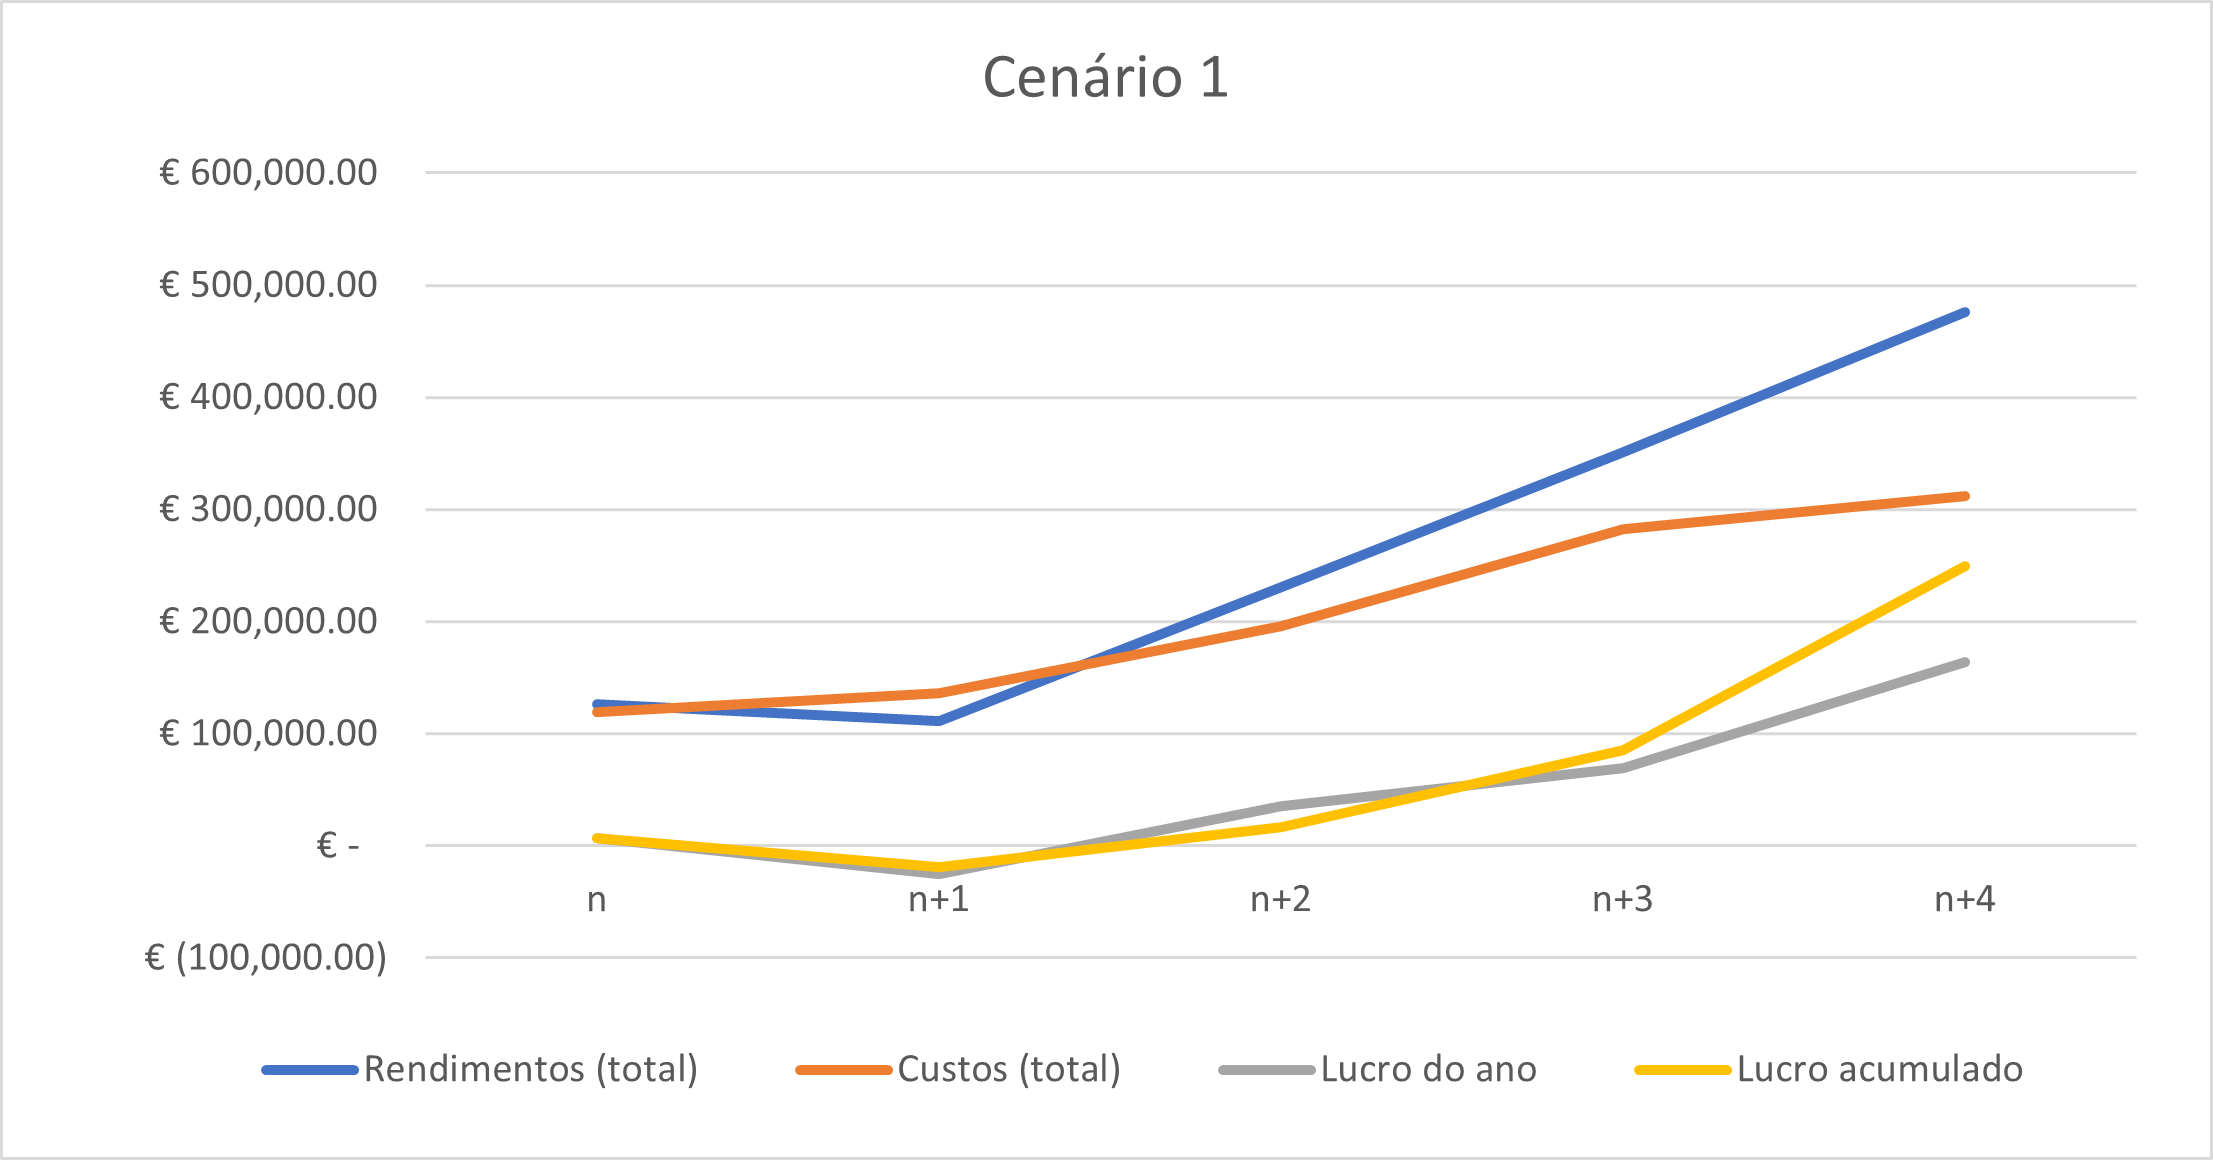
\includegraphics[width = 90mm]{img/graphs/ppin_graph_1.png}
  \caption{Gráfico ilustrativo das previsões a nível financeiro para o cenário descrito como otimista}
\end{figure}

\vspace{-0.5em}

\begin{figure}[ht]
  \centering
  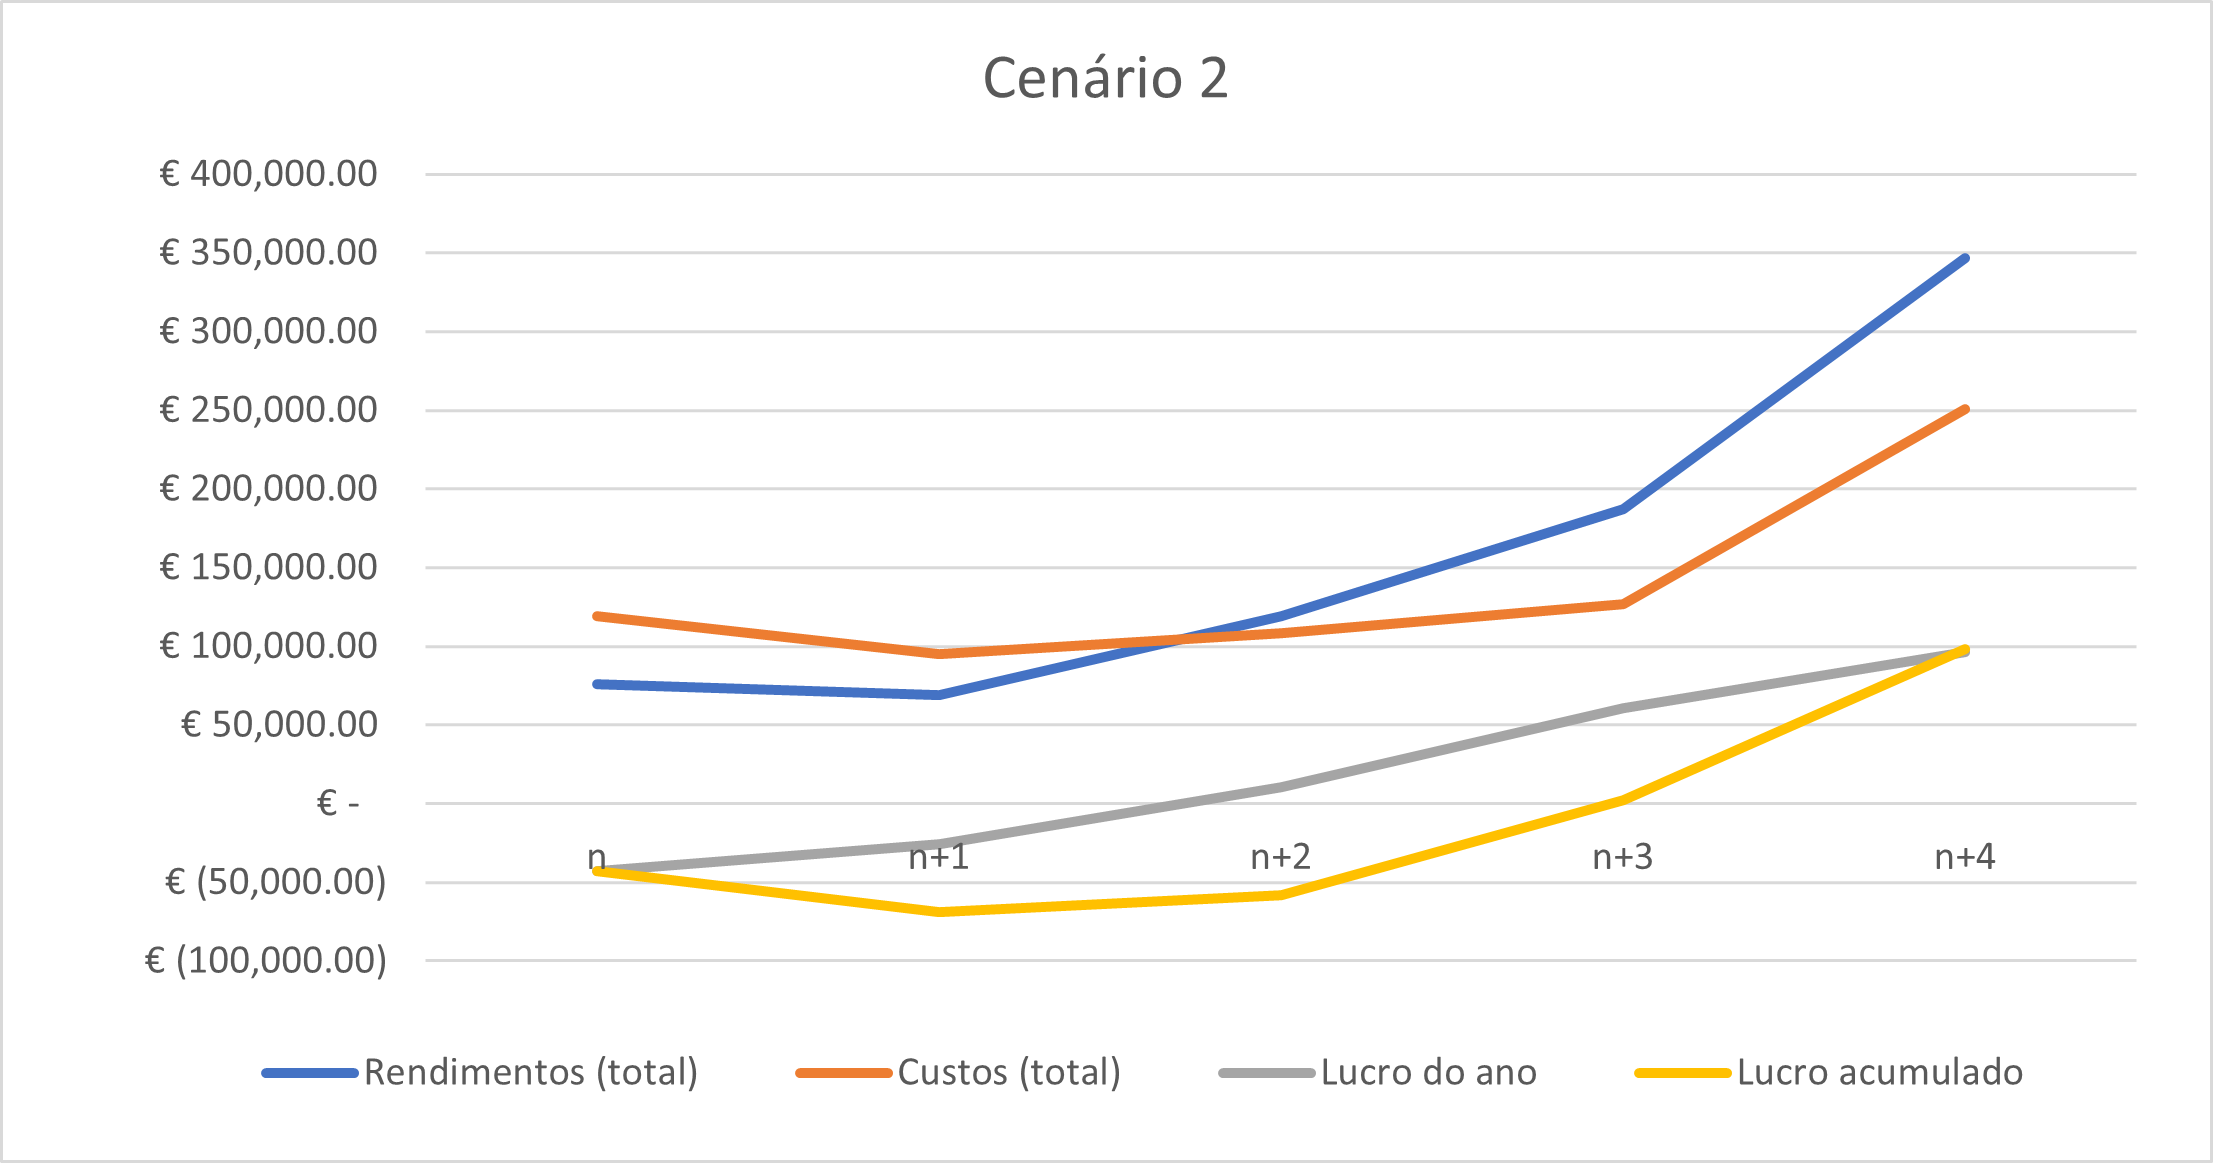
\includegraphics[width = 90mm]{img/graphs/ppin_graph_2.png}
  \caption{Gráfico ilustrativo das previsões a nível financeiro para o cenário descrito como neutro}
\end{figure}

\vspace{-0.5em}

\begin{figure}[ht]
  \centering
  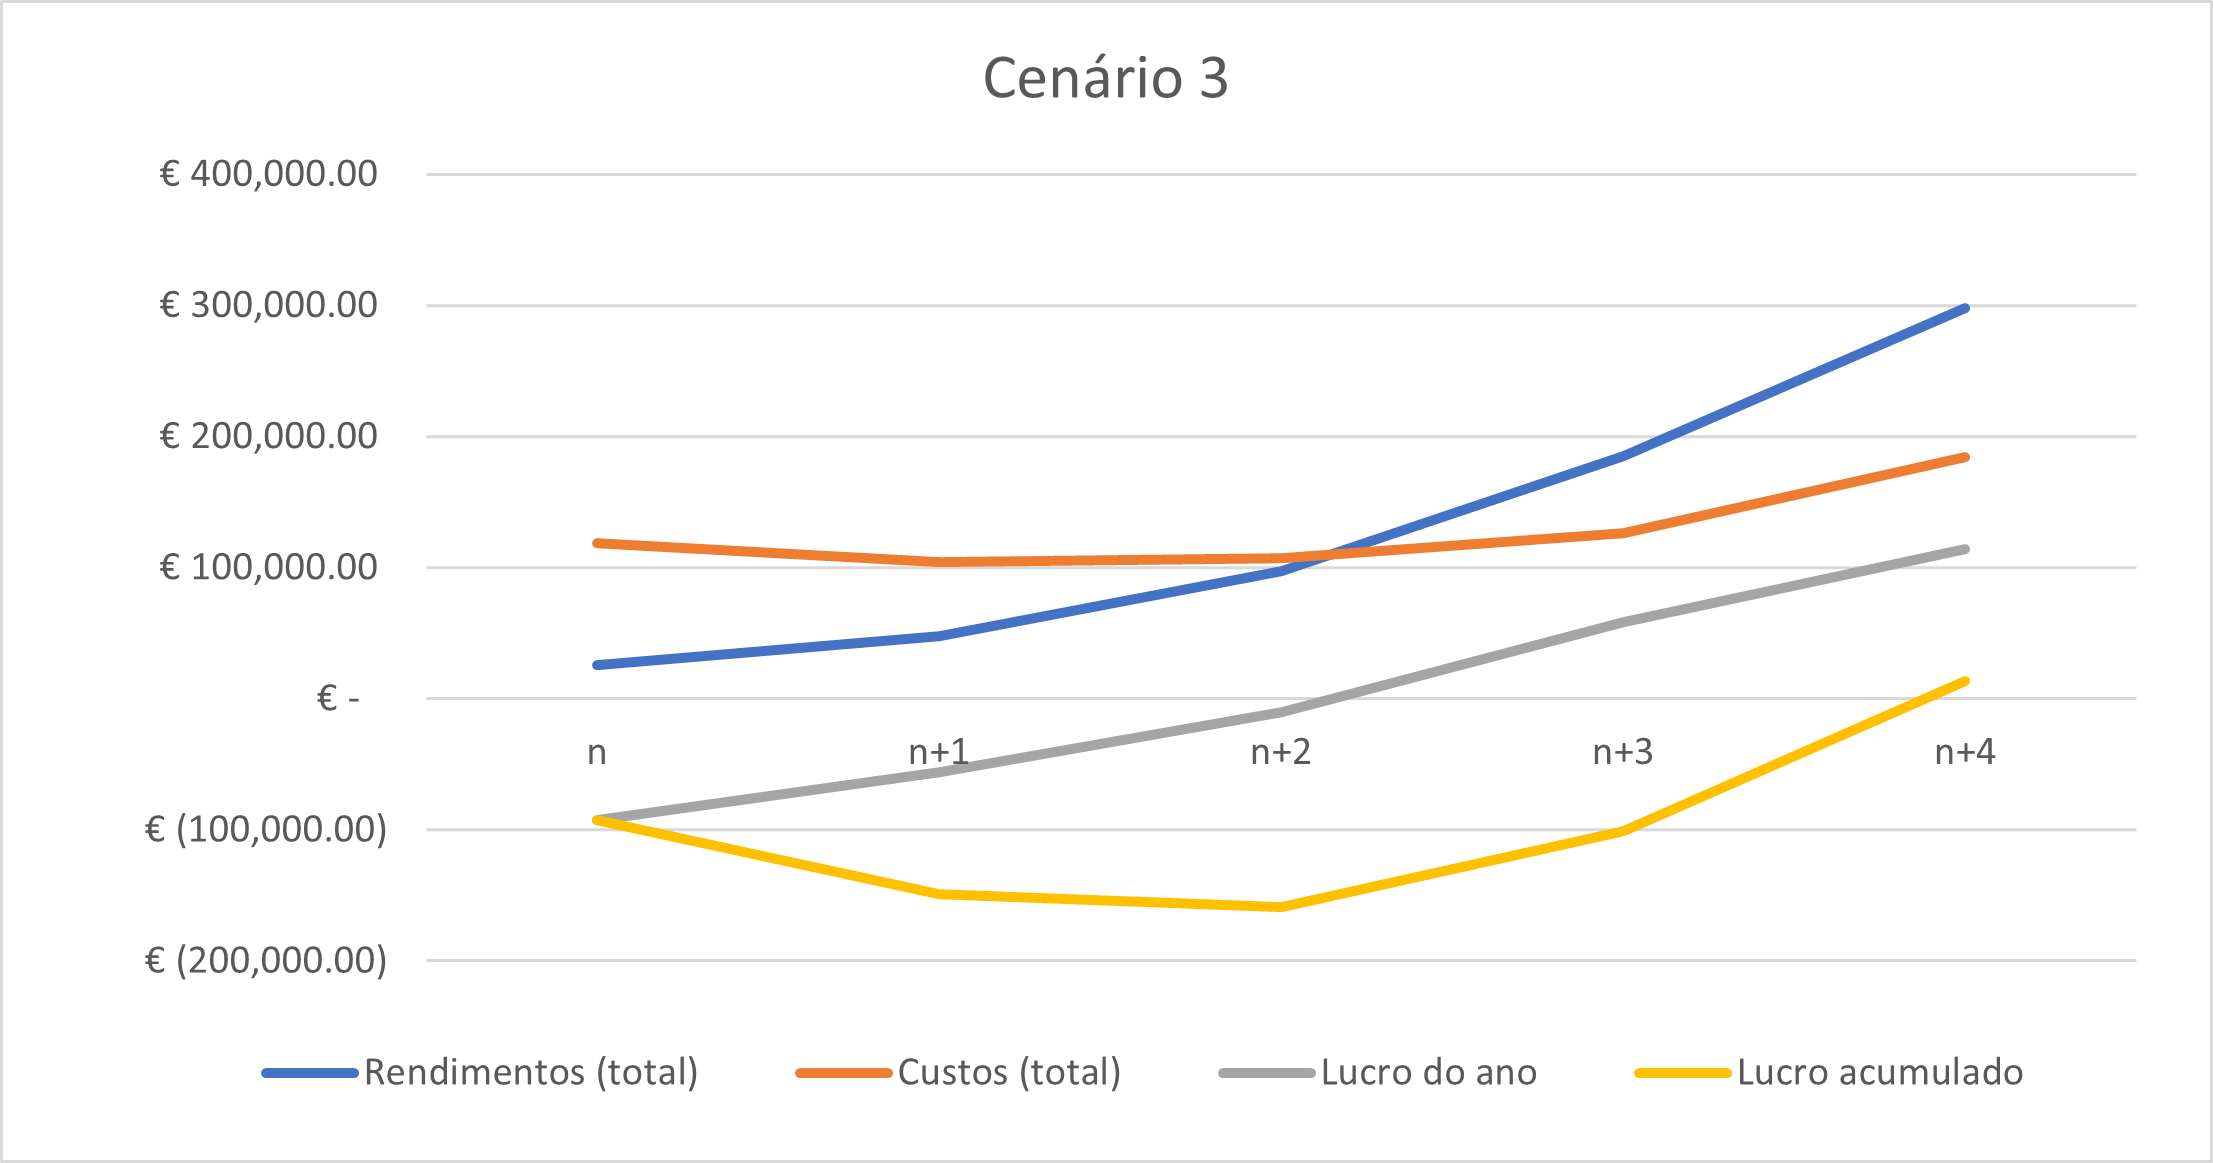
\includegraphics[width = 90mm]{img/graphs/ppin_graph_3.png}
  \caption{Gráfico ilustrativo das previsões a nível financeiro para o cenário descrito como pessimista}
\end{figure}


\chapter{Diário de bordo}

Neste anexo são apresentados as datas e os resumos das reuniões e do trabalho desenvolvido pelos membros do grupo, do momento de sua formação à entrega do trabalho final.

As reuniões realizaram-se de forma remota dada a situação pandémica, durante as aulas da unidade curricular PPIN e também através de chamadas na aplicação Discord, onde foi criado um servidor para comunicação informal entre reuniões, através de mensagens.

\section{Planeamento}

{
\renewcommand{\arraystretch}{1.5}
\begin{tabular}{@{~~} !{\foo} >{\raggedright\arraybackslash}l p{130mm}}
\addlinespace[1.5ex]
\textbf{22/03/2021} & Formação do grupo, após demostração de interesse por parte de todos os membros, no desenvolvimento de um projeto com ênfase no ambiente. \\
\textbf{25/03/2021} & Primeira reunião após a formação do grupo. Foram expostas as opiniões e vontades individuais de cada um frente ao projeto, assim como a primeira discussão sobre ideias de temas a serem escolhidos. Ficou acordado entre os membros de desenvolver uma elaboração das ideias individuais de tema, para na próxima reunião ser realizada uma apresentação interna e decisão do tema. \\
\textbf{29/03/2021} & Foram apresentados possíveis temas, por três integrantes do grupo: Desflorestação, Recolha de Resíduos e Separação de Resíduos com Inteligência Artificial. Após avaliação e votação de todos foi escolhida a Recolha de Resíduos.\\
\textbf{01/04/2021} & Primeira apresentação do tema, em aula.\\
\textbf{05/04/2021} & Reunião em seguimento da apresentação, debateu-se as críticas dos colegas, e possíveis soluções a estas. Foram separadas tarefas relativas a pesquisa de tecnologias semelhantes a proposta do trabalho, já existentes, para serem debatidas na próxima reunião.\\
\textbf{12/04/2021} & Em reunião foram revisadas as pesquisas sobre tecnologias e concorrência existentes. Assim como a discussão sobre legislações vigentes, e diferença de funcionamento do recolhimento de lixo em diferentes concelhos.\\
\textbf{17/04/2021} & Reunião final da fase de planeamento: foi analisado o desempenho desta fase e feito do planeamento da próxima fase. O formato do projeto foi estabelecido e as próximas etapas seriam a pesquisa aprofundada e desenvolvimento dos detalhes do funcionamento do produto por exemplo como seria a aplicação e se seria usada uma etiqueta NFC ou outra tecnologia. \\
\end{tabular}
}

\section{Desenvolvimento - Desafios Tecnológicos}

{
\renewcommand{\arraystretch}{1.5}
\begin{tabular}{@{~~} !{\foo} >{\raggedright\arraybackslash}l p{130mm}}
\addlinespace[1.5ex]
\textbf{21/04/2021} & Reunião inicial da fase, foram debatidas as diferentes possíveis tecnologias a serem usadas como de travas elétricas nos caixotes, etiquetas NFC's vs QR codes, dispositivos para pesagem de lixo. Foram separadas essas tecnologias para serem pesquisadas mais a fundo pelos membros e serem apresentadas na próxima reunião. \\
\textbf{24/04/2021} & Foram apresentadas em reunião os pontos pesquisados, e decididas as tecnologias a serem usadas. Assim como desenvolvido o plano de ação para a próxima fase.
\end{tabular}
}

\section{Desenvolvimento - Análise de Sustentabilidade}

{
\renewcommand{\arraystretch}{1.5}
\begin{tabular}{@{~~} !{\foo} >{\raggedright\arraybackslash}l p{130mm}}
\addlinespace[1.5ex]
\textbf{27/04/2021} & Reunião inicial da fase: foram debatidos os planos de negócio do projeto sua relação com as entidades responsáveis, e o funcionamento distinto relativo ao método de recolha de lixo nos diferentes concelhos. Ficou decidido que seria pesquisado melhor as vantagens e desvantagens das ideias apresentadas e seria decidido na próxima reunião o funcionamento. \\
\textbf{01/05/2021} & Foram apresentados os resultados do trabalho no tempo entre a última reunião. Ficou decidido o modelo final de negócios e da comunicação com as entidades. \\
\textbf{07/05/2021} & Reunião final da etapa de Desenvolvimento: foi feita uma avaliação geral do projeto até então. Uma formalização das ideias no primeiro modelo deste relatório e uma preparação para a etapa de realização. 
\end{tabular}
}

\section{Realização}

{
\renewcommand{\arraystretch}{1.5}
\begin{tabular}{@{~~} !{\foo} >{\raggedright\arraybackslash}l p{130mm}}
\addlinespace[1.5ex]
\textbf{10/05/2021} & Foram dividias as tarefas relativas a realização do relatório final, da apresentação e dos trabalhos envolvidos nestes.\\
\textbf{13/05/2021} & Durante a reunião durante a aula foi discutida a ideia de enviar um inquérito através do e-mail dinâmico. Todos os membros do grupo concordaram que seria benéfico para a realização do projeto.\\
\textbf{15/05/2021} & Reunião para a elaboração do inquérito. Ficou decidido que seriam dez questões, relativas aos hábitos dos estudantes quanto a reciclagem e sua disposição para aderir ao projeto.\\
\textbf{16/05/2021} & Envio do inquérito através do e-mail dinâmico\\
\textbf{19/05/2021} & Reunião pré apresentação final: foi revisto o resultado do inquérito, a trabalho desenvolvido e foi dividido o que cada membro iria falar na apresentação.\\
\textbf{20/05/2021} & Apresentação final do trabalho \\
\end{tabular}
}

\chapter{Mockups do protótipo}
\label{ch:anexo-mockups}

Apresentam-se de seguida os mockups do protótipo da aplicação móvel e da web app.

\subsubsection{Aplicação móvel}

\begin{figure}[h!]
    \centering
    
    \begin{subfigure}[t]{0.33\textwidth}
        \centering
        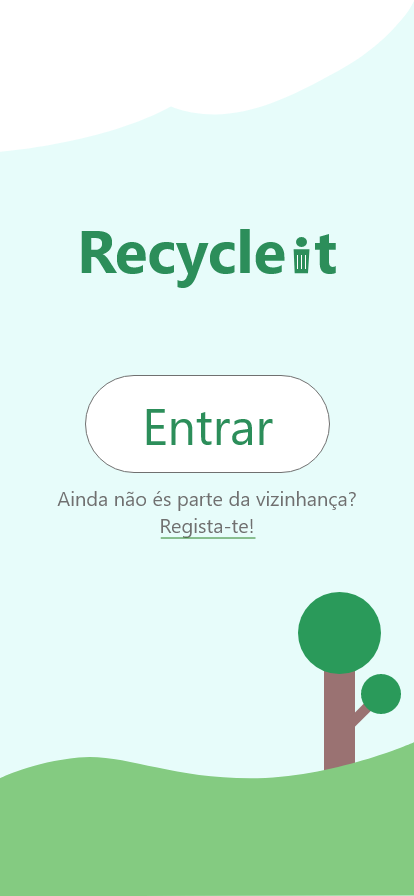
\includegraphics[width=52mm]{img/mockups/tlmv-1.png}
        \caption{Ecrã de entrada}
    \end{subfigure}%
    \begin{subfigure}[t]{0.33\textwidth}
        \centering
        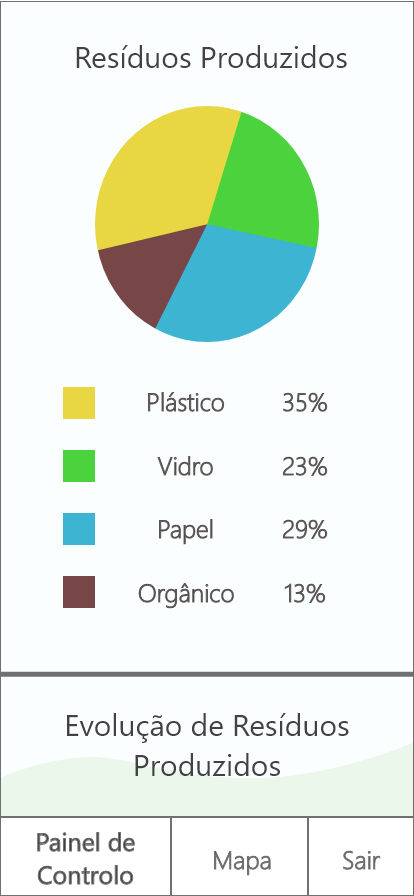
\includegraphics[width=52mm]{img/mockups/tlmv-2.png}
        \caption{Consulta do lixo produzido}
    \end{subfigure}%
    \begin{subfigure}[t]{0.33\textwidth}
        \centering
        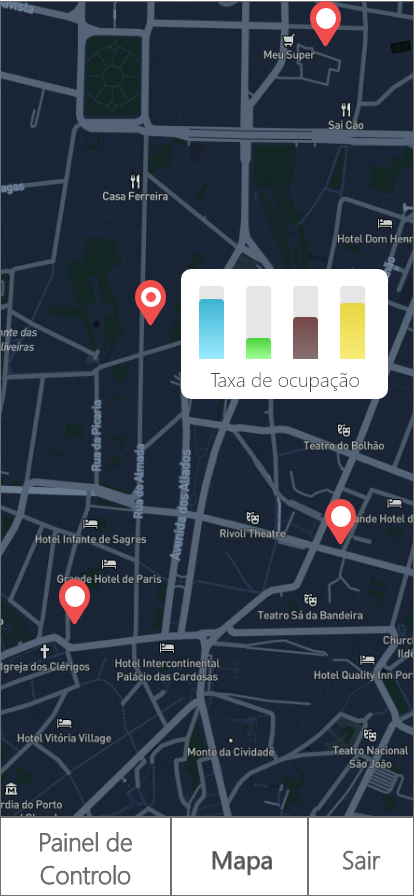
\includegraphics[width=52mm]{img/mockups/tlmv-3.png}
        \caption{Consulta dos ecopontos}
    \end{subfigure}
    
    \caption{Mockups do protótipo da aplicação móvel}
\end{figure}

\newpage

\subsubsection{Web app}

\begin{figure}[h!]
    \centering
    
    \begin{subfigure}[t]{0.99\textwidth}
        \centering
        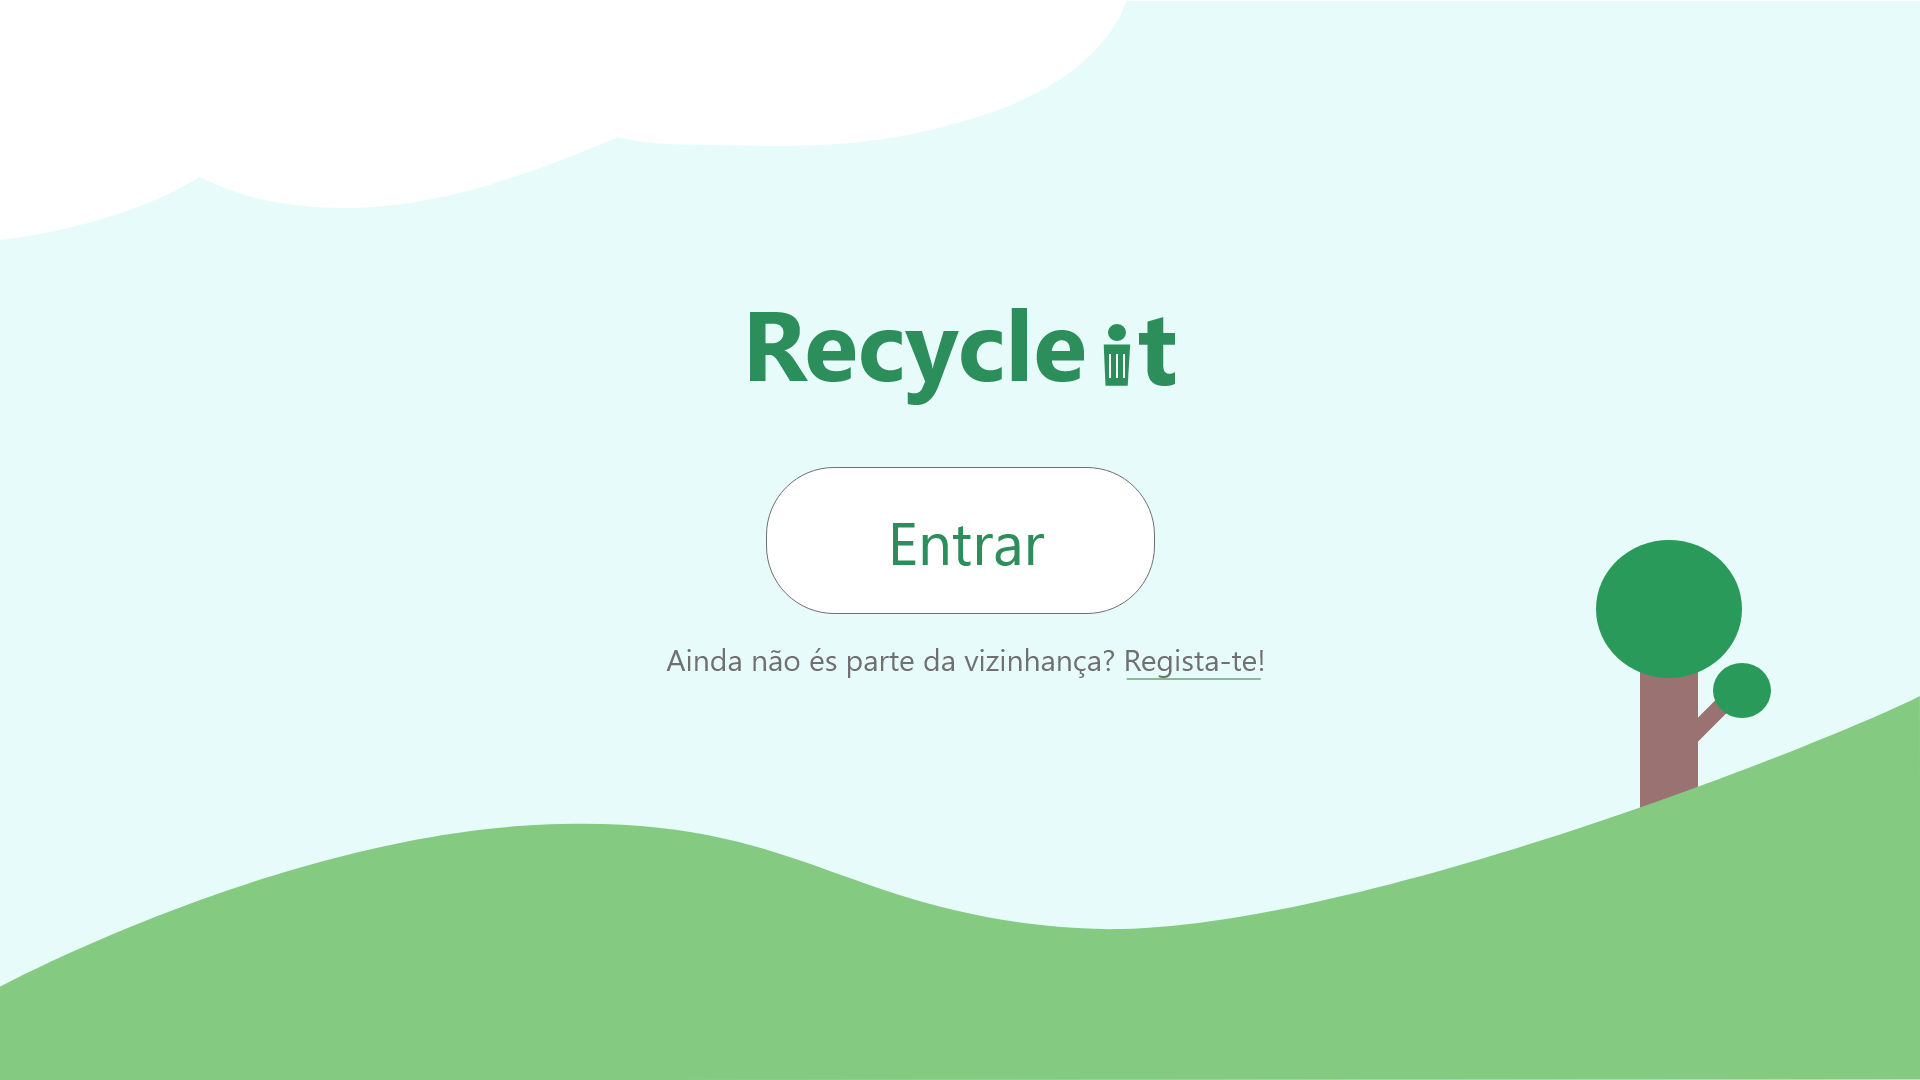
\includegraphics[width=120mm]{img/mockups/web-1.png}
        \caption{Ecrã de entrada}
    \end{subfigure}
    \begin{subfigure}[t]{0.99\textwidth}
        \centering
        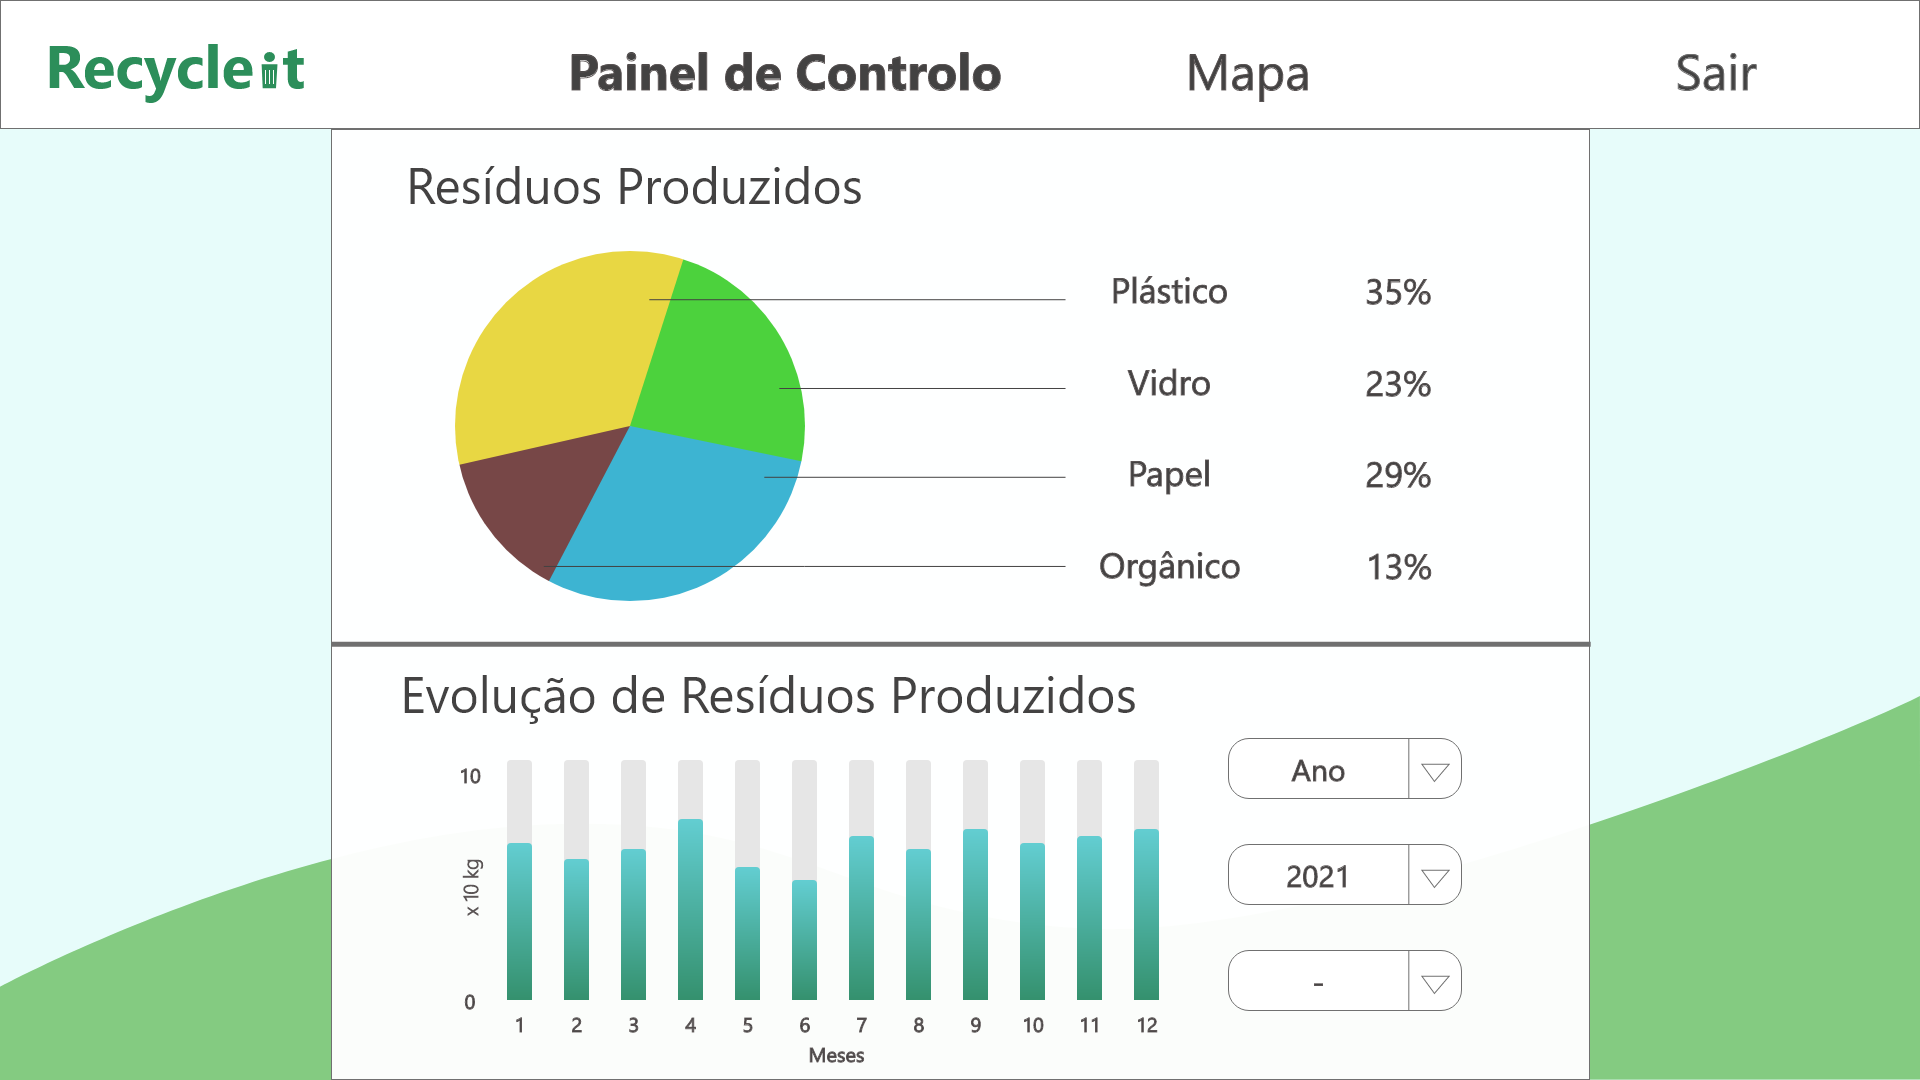
\includegraphics[width=120mm]{img/mockups/web-2.png}
        \caption{Consulta do lixo produzido}
    \end{subfigure}
    \begin{subfigure}[t]{0.99\textwidth}
        \centering
        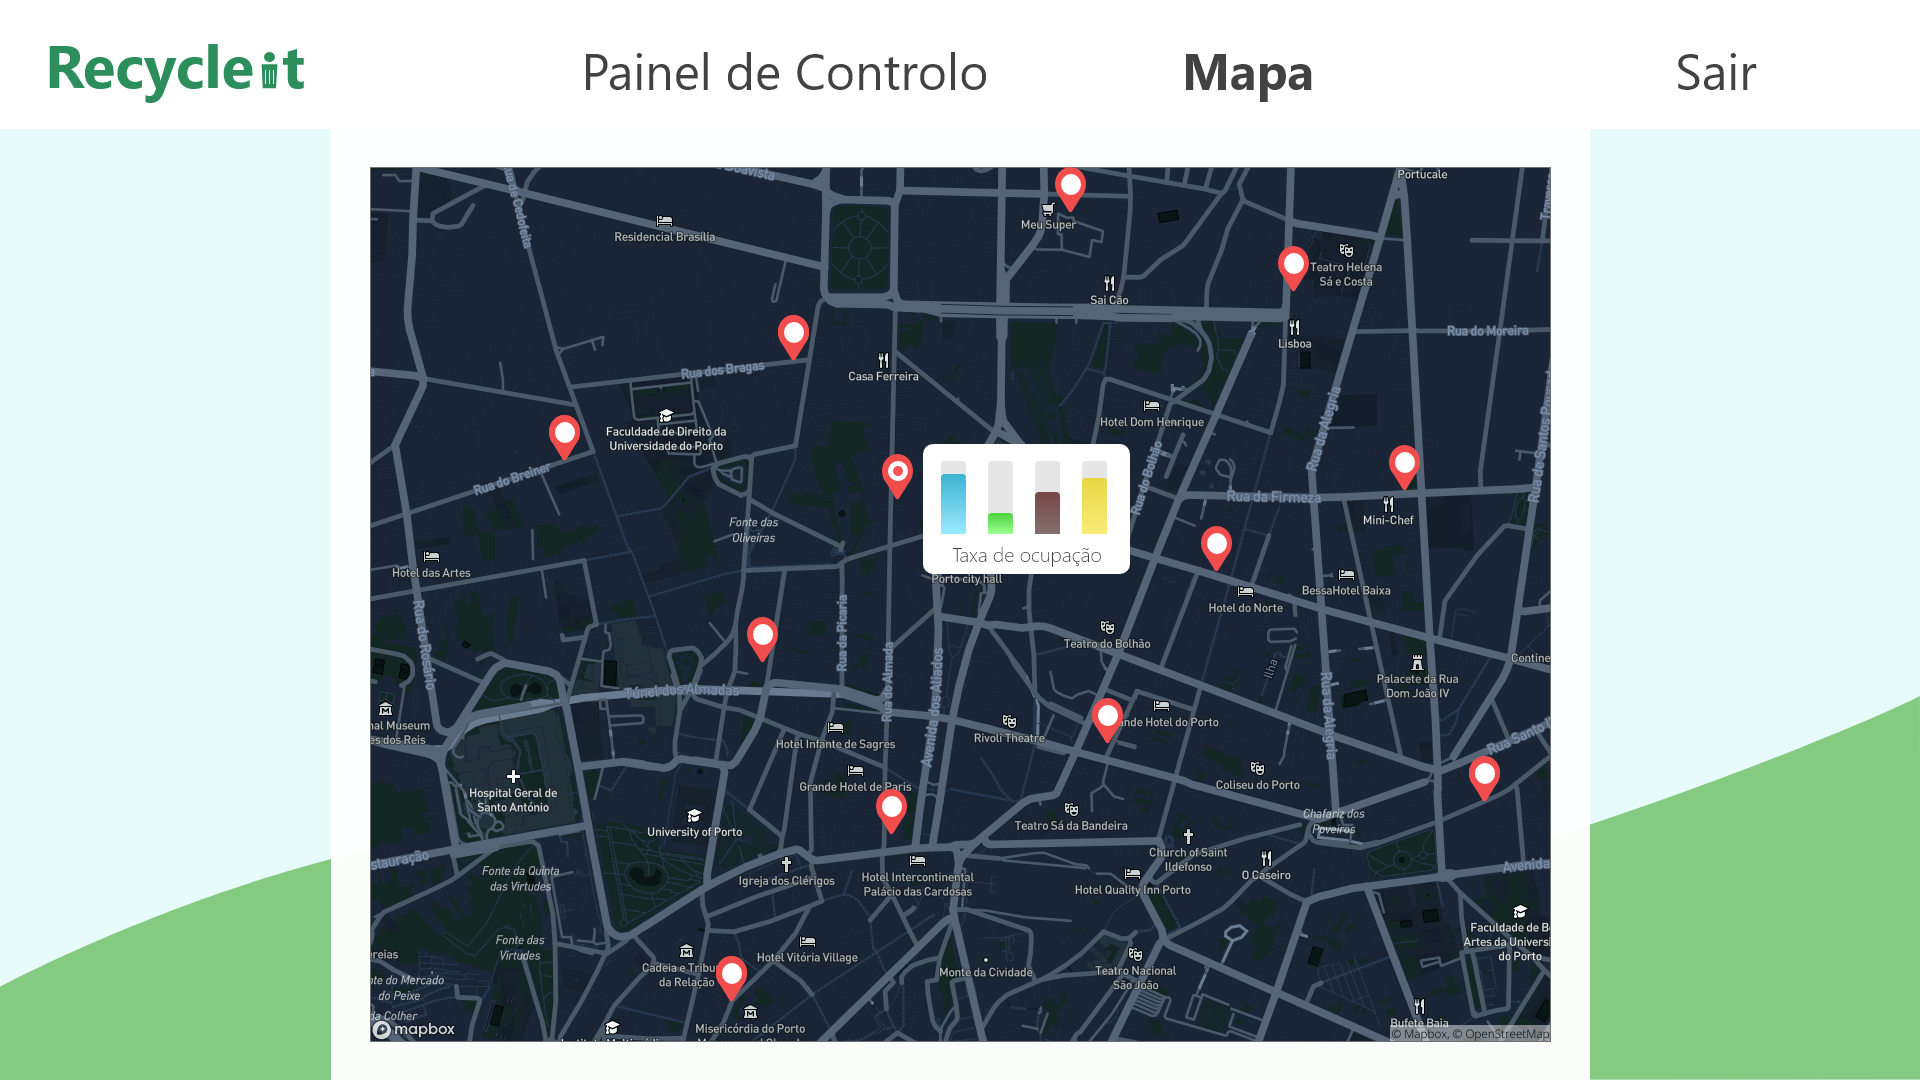
\includegraphics[width=120mm]{img/mockups/web-3.png}
        \caption{Consulta dos ecopontos}
    \end{subfigure}
    
    \caption{Mockups do protótipo da web app}
\end{figure}

\chapter{Media}

Segue-se o \textit{media} deste projeto, que consiste nas várias versões do logótipo. A cor verde é trocada por branco (e a cor branca é trocada por transparência, como nos traços do caixote de lixo no "i") quando é necessário colocar o logótipo sobre um fundo não-branco.

\subsubsection{Logótipo completo}

\begin{center}
    
\includegraphics[scale=2.0]{img/recycle-it-full.png}
\end{center}

\subsubsection{Logótipo pequeno}

\begin{center}
    
\includegraphics[scale=2.0]{img/recycle-it.png}
\end{center}

\end{appendices}

\end{document}
